\documentclass[11pt,a4paper]{article}
\usepackage{amsmath,amssymb,amsthm}
\usepackage[margin=2.5cm]{geometry}
\usepackage{graphicx}
\usepackage{xcolor}
\usepackage{booktabs}
\usepackage{longtable}
\usepackage{tabularx}
\usepackage{adjustbox}
\usepackage{enumitem}
\usepackage{microtype}
\usepackage{tcolorbox}
\usepackage[numbers,sort&compress]{natbib}
\usepackage[
    colorlinks=true,
    linkcolor=blue!55!black,
    citecolor=blue!45!black,
    urlcolor=blue!55!black,
    bookmarks=true,
    bookmarksnumbered=true,
    unicode=true
]{hyperref}

\geometry{a4paper, top=2.5cm, bottom=2.5cm, left=2.5cm, right=2.5cm}

\widowpenalty=10000
\clubpenalty=10000
\emergencystretch=3em

% ---------- theorem environments ----------
\theoremstyle{plain}
\newtheorem{theorem}{Theorem}[section]
\newtheorem{proposition}[theorem]{Proposition}
\newtheorem{lemma}[theorem]{Lemma}
\newtheorem{corollary}[theorem]{Corollary}
\newtheorem{conjecture}{Conjecture}[section]
\theoremstyle{definition}
\newtheorem{definition}[theorem]{Definition}
\newtheorem{example}[theorem]{Example}
\newtheorem{axiom}[theorem]{Axiom}
\theoremstyle{remark}
\newtheorem{remark}[theorem]{Remark}

% ---------- macros ----------
\newcommand{\ket}[1]{\lvert #1\rangle}
\newcommand{\bra}[1]{\langle #1\rvert}
\newcommand{\braket}[2]{\langle #1\rvert #2\rangle}
\newcommand{\Pz}{\mathbb{P}}
\newcommand{\Nn}{\mathbb{N}}
\newcommand{\Zz}{\mathbb{Z}}
\newcommand{\Qq}{\mathbb{Q}}
\newcommand{\Rr}{\mathbb{R}}
\newcommand{\Cc}{\mathbb{C}}
\newcommand{\Fock}{\mathcal{F}}
\newcommand{\Hil}{\mathcal{H}}
\newcommand{\Nhat}{\widehat{N}}
\newcommand{\Hmax}{\widehat{\mathcal{H}}}
\DeclareMathOperator{\Tr}{Tr}
\DeclareMathOperator{\spec}{spec}
\DeclareMathOperator{\Gal}{Gal}
\DeclareMathOperator{\Frob}{Frob}

\begin{document}

% Body starts with TOC; cover is merged separately as page 0.
\tableofcontents
\newpage

% =====================================================================
% SECTION 1: Introduction and method  +  SECTION 2: Arithmetic sector
% =====================================================================

\section*{Abstract}
\noindent
This document is a rigorous reconstruction of the ``prime-spectral framework'' developed in a
forty-eight-turn source conversation, in which the statistical mechanics of a free Bose gas of
``primons'' (one-particle energies $\log p$, $p$ ranging over the rational primes) was advanced as
the arithmetic core of a unified picture of quantum gravity, time, and the arrows of time. Our
procedure is threefold. First, we \emph{elevate} every statement that admits a precise formulation:
the primon Hilbert space is defined as $\ell^{2}$ of the free commutative monoid on the primes,
sidestepping the nonseparability of naive infinite tensor products; the primon Hamiltonian is
proved self-adjoint with simple spectrum $\hbar\omega_{0}\log n$; the partition function is
identified with the Riemann zeta function; the exponential state-counting law
$N(E)=\lfloor e^{E/\hbar\omega_{0}}\rfloor$ is given its correct name, a \emph{Hagedorn spectrum}
with critical temperature $T_{H}=\hbar\omega_{0}/k_{B}$; and the ``thermodynamic cascade into
composite states'' is grounded in the Hardy--Ramanujan and Erd\H{o}s--Kac theorems. Second, we
\emph{repair} the central gaps: the frozen-Hamiltonian problem (the diagonal primon Hamiltonian
admits no transitions), the false identification of composite integers with entangled states
(occupation-basis states are product states across every prime-mode bipartition), and the
overstrong no-recurrence claim (exact periodicity is indeed forbidden by the
$\Qq$-linear independence of prime logarithms, but approximate recurrence survives in every
finite truncation). Third, we \emph{demote} to an explicit, falsifiable conjecture register every
claim whose proof is out of reach, from the zeta/black-hole partition-function identification to
the Galois--Langlands dictionary for the Standard Model. The result is a framework whose
mathematical core is now theorem-grade, whose analogies are tightened to citable results, and
whose remaining ambitions are stated with enough precision to be attacked or refuted.

\bigskip

\section{Introduction: Source, Method, and Results}\label{sec:intro}

\subsection{The source conversation}

The source material is a shared conversation (48 turns) in which a user and an assistant
co-developed a speculative but internally ambitious framework: that the prime numbers, through the
primon gas of Julia~\cite{julia1990} and Spector~\cite{spector1998}, supply the quantum-mechanical
spectrum of the near-singularity gravitational field, that the Riemann zeta function is the
gravitational partition function, and that the entire architecture of time---its problem, its
arrow, its block-universe metaphysics, and its impossibility of cycles---follows from the
arithmetic of the integers. The conversation drew on reported 2025--2026 developments linking
conformal primon gases to black-hole interiors~\cite{hartnollyang2026}, on the philosophical
literature of time's arrow~\cite{carroll2010,wallace2017,price1996}, and on first-person
metaphysics~\cite{hellie2013,hare2009,conitzer2019}. It culminated in claims that Gaussian primes
extend the framework to five dimensions, that the Absolute Galois group plays the role of a grand
unified symmetry, and that gravity is an entropic, $1/N$-suppressed collective effect.

Taken verbatim, the conversation alternates between genuine mathematics, physics speculation, and
rhetorical overreach. That alternation is precisely what makes it worth reconstructing: the
skeleton is sound and unusually coherent, while the joints are loose. The present document
keeps the skeleton, tightens every joint, discards nothing that can be saved by honest
reformulation, and labels everything else.

\subsection{Method: elevate, repair, demote}\label{sec:method}

Every substantive claim in the source was subjected to one of three treatments.

\begin{enumerate}[leftmargin=1.6em]
\item \textbf{Elevate.} If a claim has a precise mathematical formulation and a proof, it is
stated as a theorem, lemma, or proposition with its proof or an exact citation. Examples: the
$\Qq$-linear independence of $\{\log p\}$; the identification of the partition function with
$\zeta$; the Hagedorn asymptotics; the positive-definiteness of the Page--Wootters clock kernel;
the exact state-counting identity $\log N(E)=E/\hbar\omega_{0}+O(1)$.
\item \textbf{Repair.} If a claim is right in spirit but wrong in mechanism, the mechanism is
replaced and the repaired claim is re-proved. Three repairs dominate this document:
(i)~the diagonal primon Hamiltonian cannot drive the claimed ``cascade into composite states'',
so a multiplicative transition sector (multiplication operators $M_{n}$ and a hopping dynamics
on the \emph{prime lattice}) is introduced in Section~\ref{sec:dynamics};
(ii)~composite integers are \emph{not} entangled states---the occupation basis is a product
basis---so arithmetic entanglement is redefined across prime-mode bipartitions in
Section~\ref{sec:entangle}, and the ``arithmetic holism'' that resolves Bell's trilemma is
relocated from single integers to superpositions;
(iii)~the ``universe cannot repeat'' claim conflated exact periodicity, Poincar\'e recurrence,
and dynamical return; these are separated in Section~\ref{sec:recurrence} into one theorem and
two counterexamples.
\item \textbf{Demote.} If a claim is plausible, well-formed, and beyond current proof
technology, it is restated as a numbered conjecture with evidence, dependencies, and a
falsifier. Twelve conjectures ($\mathsf{C1}$--$\mathsf{C12}$) are consolidated in
Section~\ref{sec:register}. The guiding rule is that a conjecture must be \emph{attackable}:
each one carries at least one specified route to confirmation or refutation.
\end{enumerate}

An audit trail of the corrections is given in Appendix~\ref{app:corrections}; it lists each
original claim, its repaired or demoted status, and the pointer to the section where the
treatment occurs. Nothing in the source ambition is silently dropped: where a claim is rejected
outright (for example, that the Hamiltonian $H_{P}=\hbar\omega_{0}\log\Nhat$ by itself ``drives
transitions into composite integer states''), the rejection is argued, and the surviving
content is carried forward under its own name.

\subsection{Summary of results}

The reconstruction yields a layered structure. The \emph{mathematical floor} (all theorem-grade)
consists of: the arithmetic Hilbert space $\Hil_{\mathcal{A}}=\ell^{2}(\Nn,\times)$
(Section~\ref{sec:arithmetic}); the self-adjoint primon Hamiltonian with simple spectrum
$\hbar\omega_{0}\log n$; the partition function $Z(\beta)=\zeta(\beta\hbar\omega_{0})$ with
Hagedorn temperature $T_{H}=\hbar\omega_{0}/k_{B}$; the exact counting law
$\log N(E)=E/\hbar\omega_{0}+O(1)$; the Erd\H{o}s--Kac statistics of the microcanonical
ensemble; the isometric representation $n\mapsto M_{n}$ of the multiplicative monoid on
$\Hil_{\mathcal{A}}$; the phase-incommensurability theorem forbidding exact periodicity; the
Bohr almost-periodicity of the zeta clock's correlation kernel; and the product-state theorem
that repairs the entanglement story. The \emph{conjectural superstructure} consists of the
twelve register entries, of which the deepest are $\mathsf{C1}$ (the zeta/black-hole
identification), $\mathsf{C3}$ (the arithmetic holographic bound), $\mathsf{C4}$ (thermalization
on the prime lattice), and $\mathsf{C9}$ (the Galois--gauge dictionary).

The philosophical theses of the source---eternalism with perspectival observers, an extrinsic
arrow grounded in arithmetic state-counting, derivative causality, and the rejection of
superdeterminism---survive the reconstruction in \emph{conditional} form: they are
well-defined consequences of the conjectural superstructure, and they are marked as
interpretive rather than theorem-grade wherever the mathematics cannot carry them
(Section~\ref{sec:philosophy}).

\section{The Arithmetic Sector}\label{sec:arithmetic}

This section fixes the foundational objects. Everything here is elementary but must be stated
carefully, because the source conversation (and part of the physics literature) informally
writes the primon Fock space as an infinite tensor product, an object that is \emph{not}
separable and is the wrong home for the theory. The repair is cheap and clarifying.

\subsection{The arithmetic Hilbert space}

Let $\Pr=\{2,3,5,\dots\}$ denote the rational primes. Let
\begin{equation}\label{eq:monoid}
\mathcal{F}\;=\;\Bigl\{k\colon \Pr\to\Nn \;:\; k_{p}\neq 0 \text{ for only finitely many } p\Bigr\}
\end{equation}
be the free commutative monoid on the primes. By the fundamental theorem of arithmetic, the
map $\mathcal{F}\to\Nn_{\geq 1}$, $k\mapsto \prod_{p}p^{k_{p}}$, is a monoid isomorphism
between $(\mathcal{F},+)$ and $(\Nn_{\geq 1},\times)$, where $+$ denotes componentwise addition
of occupation vectors. This single classical theorem is the load-bearing wall of the entire
framework: it is what makes ``states of the arithmetic universe'' and ``positive integers''
the same bookkeeping.

\begin{definition}[Arithmetic Hilbert space]\label{def:hilbert}
The \emph{arithmetic Hilbert space} is
\begin{equation}
\Hil_{\mathcal{A}}\;=\;\ell^{2}(\mathcal{F})\;\cong\;\ell^{2}(\Nn_{\geq 1}),
\end{equation}
with orthonormal basis $\{\ket{k}\}_{k\in\mathcal{F}}$, written $\ket{n}$ for
$n=\prod_{p}p^{k_{p}}$ when no confusion arises. Each prime $p$ defines a \emph{mode} with
occupation counter
\begin{equation}
\hat n_{p}\ket{k}=k_{p}\ket{k},
\end{equation}
a self-adjoint operator with spectrum $\Nn$.
\end{definition}

\begin{remark}[Why not an infinite tensor product?]
The source writes $\Fock_{\Pr}=\bigotimes_{p\in\Pr}\Fock_{p}$ with one bosonic oscillator per
prime. The literal von Neumann infinite tensor product of the $\ell^{2}(\Nn)$ over a countably
infinite index set is nonseparable, and its physically relevant separable subspaces depend on
a choice of reference vector. Definition~\ref{def:hilbert} achieves the intended object
directly: $\ell^{2}$ of the countable basis $\mathcal{F}$ is separable, and the tensor
factorization over any \emph{finite} set of modes is available whenever needed
(Proposition~\ref{prop:productstructure}). This is the first, and easiest, instance of the
general principle of this reconstruction: replace informal infinite constructions by the
countable objects they were meant to describe.
\end{remark}

For each prime $p$ the standard bosonic ladder operators act on the $p$-mode: on basis vectors
\begin{equation}
a_{p}^{\dagger}\ket{k}=\sqrt{k_{p}+1}\,\ket{k+e_{p}},
\qquad
a_{p}\ket{k}=\sqrt{k_{p}}\,\ket{k-e_{p}},
\end{equation}
where $e_{p}$ is the unit occupation vector, and $[a_{p},a_{q}^{\dagger}]=\delta_{pq}$ holds
on the dense span of basis vectors. The total particle number is
$\Nhat_{\mathrm{tot}}=\sum_{p}\hat n_{p}$, self-adjoint on
$\{\psi:\sum_{p}k_{p}^{2}|\psi_{k}|^{2}<\infty\}$.

\subsection{The multiplicative number operator and the primon Hamiltonian}

The source's central operator is the \emph{multiplicative number operator}, whose eigenvalue on
$\ket{k}$ is the integer $n=\prod_{p}p^{k_{p}}$ itself. We define it together with the
Hamiltonian it generates.

\begin{definition}[Multiplicative number operator; primon Hamiltonian]\label{def:hamiltonian}
The \emph{multiplicative number operator} $\Nhat$ is the diagonal operator
\begin{equation}
\Nhat\ket{k}=\Bigl(\prod_{p}p^{k_{p}}\Bigr)\ket{k},
\end{equation}
self-adjoint on its maximal domain. The \emph{primon Hamiltonian} is
\begin{equation}\label{eq:primonH}
H_{P}\;=\;\hbar\omega_{0}\log\Nhat
\;=\;\hbar\omega_{0}\sum_{p\in\Pr}(\log p)\,\hat n_{p},
\qquad \omega_{0}>0,
\end{equation}
where the equality of the two expressions is pointwise on basis vectors and extends by
closure.
\end{definition}

Equation~\eqref{eq:primonH} exhibits $H_{P}$ as a \emph{free Bose gas} whose one-particle
spectrum is $\{\log p:p\in\Pr\}$: each prime is one species of elementary excitation (a
\emph{primon}), and a many-body state $\ket{n}$ has energy equal to the logarithm of the
integer it represents. This is Julia's primon gas~\cite{julia1990}, cleaned of its informal
packaging.

\begin{theorem}[Self-adjointness, spectrum, and simplicity]\label{thm:spectrum}
$H_{P}$ is self-adjoint and nonnegative. Its spectrum is the pure point set
\begin{equation}
\spec(H_{P})=\overline{\{\hbar\omega_{0}\log n:n\in\Nn_{\geq 1}\}},
\end{equation}
a discrete set whose only accumulation point is $+\infty$; it has no finite accumulation
point. Every eigenvalue $\hbar\omega_{0}\log n$ is
\emph{simple}: $\log m=\log n$ if and only if $m=n$. The ground state is the vacuum
$\ket{1}$ with eigenvalue $0$, and it is unique.
\end{theorem}

\begin{proof}
Under the unitary $U\colon\Hil_{\mathcal{A}}\to\ell^{2}(\Nn_{\geq 1})$,
$U\ket{k}=\ket{n}$ (unitary by the fundamental theorem of arithmetic),
$H_{P}$ becomes multiplication by the real sequence
$a_{n}=\hbar\omega_{0}\log n$. Multiplication by a real-valued sequence is self-adjoint on its
maximal domain $\{c\in\ell^{2}:\sum_{n}a_{n}^{2}|c_{n}|^{2}<\infty\}$, and its spectrum is the
closure of $\{a_{n}\}$. Since $a_{n}\to\infty$ monotonically, the closure adds no finite
points. Simplicity: if $a_{m}=a_{n}$ with $m\neq n$, then $\log m=\log n$ forces $m=n$, a
contradiction. The ground state: $a_{n}\geq 0$ with equality only at $n=1$.
\end{proof}

Two consequences deserve emphasis because the source conversation uses both constantly.
First, the \emph{unique zero-entropy ground state} $\ket{1}$ is the multiplicative identity;
this is the rigorous content of the source's ``arithmetic floor'' and of its Janus point
claims, developed in Sections~\ref{sec:thermo} and~\ref{sec:philosophy}. Second, the
\emph{simplicity} of every level means the primon spectrum has no degeneracy whatsoever: the
integers label states one-to-one. Any degeneracy in a putative physical realization must
therefore come from sectors \emph{beyond} $H_{P}$ (for instance the Gaussian sector of
Section~\ref{sec:galois}).

\subsection{The partition function and the Hagedorn temperature}

\begin{proposition}[Partition function]\label{prop:partition}
For inverse temperature $\beta>0$,
\begin{equation}\label{eq:zetaZ}
Z(\beta)\;=\;\Tr\,e^{-\beta H_{P}}
\;=\;\sum_{n=1}^{\infty}e^{-\beta\hbar\omega_{0}\log n}
\;=\;\sum_{n=1}^{\infty}n^{-\beta\hbar\omega_{0}}
\;=\;\zeta(\beta\hbar\omega_{0}),
\end{equation}
and the series converges if and only if $\beta\hbar\omega_{0}>1$, i.e.
$T<T_{H}$, where
\begin{equation}\label{eq:hagedornT}
T_{H}\;=\;\frac{\hbar\omega_{0}}{k_{B}}
\end{equation}
is the \emph{Hagedorn temperature} of the primon gas. On the half-line $\sigma=\beta\hbar\omega_{0}>1$,
the Euler product
\begin{equation}\label{eq:eulerproduct}
\zeta(\sigma)=\prod_{p\in\Pr}\frac{1}{1-p^{-\sigma}}
=\prod_{p\in\Pr}\frac{1}{1-e^{-\beta\varepsilon_{p}}},
\qquad \varepsilon_{p}:=\hbar\omega_{0}\log p,
\end{equation}
is precisely the grand-canonical factorization of a free Bose gas into independent prime modes,
with each mode contributing the standard Bose factor. The mean occupation of mode $p$ is
\begin{equation}
\langle \hat n_{p}\rangle_{\beta}=\frac{1}{e^{\beta\varepsilon_{p}}-1}
=\frac{1}{p^{\beta\hbar\omega_{0}}-1}.
\end{equation}
\end{proposition}

\begin{proof}
The trace formula is the spectral decomposition of Theorem~\ref{thm:spectrum}; convergence at
$\sigma>1$ and the Euler product are Euler's theorems; the occupation formula is the standard
free-boson computation on each mode.
\end{proof}

The source conversation states the identification $Z=\zeta$ correctly but never names the
consequence that gives it physical teeth: the primon gas is a \emph{Hagedorn system}
\cite{hagedorn1965}. Its density of states grows exponentially in the energy, and the
partition function diverges at a finite critical temperature. In string theory this is the
famous signal that, near $T_{H}$, energy input goes into multiplying the number of light
degrees of freedom rather than into heating. The same reading applies here with total
exactness, because the counting is exactly solvable.

\begin{theorem}[Hagedorn asymptotics]\label{thm:hagedorn}
Let $k_{B}=1$ and write $T_{H}=\hbar\omega_{0}$. As $T\uparrow T_{H}$ (i.e.
$\sigma=\beta\hbar\omega_{0}\downarrow 1$):
\begin{align}
\zeta(\sigma)&=\frac{1}{\sigma-1}+\gamma+O(\sigma-1),\\
U(T):=-\frac{\partial}{\partial\beta}\log Z(\beta)
&=\frac{\hbar\omega_{0}}{\sigma-1}+O(\hbar\omega_{0})
\;=\;\frac{T\,T_{H}}{T_{H}-T}+O(T_{H}),\\
S(T):=\beta U+\log Z
&=\frac{1}{\sigma-1}-\log(\sigma-1)+O(1),\\
C(T):=\frac{dU}{dT}
&=\frac{T_{H}^{2}}{(T_{H}-T)^{2}}\,\bigl(1+O((T_{H}-T)/T)\bigr).
\end{align}
In particular the specific heat diverges as $T\uparrow T_{H}$, while the entropy diverges
only as $T/(T_{H}-T)$; energy is absorbed at nearly constant temperature.
\end{theorem}

\begin{proof}
The Laurent expansion $\zeta(\sigma)=1/(\sigma-1)+\gamma+O(\sigma-1)$ is classical
\cite{titchmarsh1986}. Then
$-\zeta'/\zeta(\sigma)=[1/(\sigma-1)^{2}+O(1)]/[1/(\sigma-1)+O(1)]=1/(\sigma-1)+O(1)$, giving
$U=\hbar\omega_{0}(-\zeta'/\zeta)(\sigma)$. Substituting $\sigma=T_{H}/T$ gives
$\sigma-1=(T_{H}-T)/T$ and the stated form. The entropy follows from
$S=\beta U+\log Z$ with $\log Z=-\log(\sigma-1)+O(1)$. Differentiating $U=T T_{H}/(T_{H}-T)$
in $T$ gives $C=T_{H}^{2}/(T_{H}-T)^{2}$ up to the stated relative error.
\end{proof}

\begin{remark}[Microcanonical reading]
Section~\ref{sec:thermo} proves the exact counting law
$\log N(E)=E/\hbar\omega_{0}+O(1)$, which says that the \emph{microcanonical} temperature
$(dS/dE)^{-1}$ equals $T_{H}$ identically, at every energy scale: the primon gas is an exactly
critical system. It never heats; it only multiplies states. This is the sharpened form of the
source's statement that ``the state space expands exponentially'': the expansion rate is not
merely large, it is \emph{uniform} in $E$, and that uniformity is what the pole of $\zeta$ at
$s=1$ encodes. The classical smooth term ``$x$'' of the prime number theorem is the same
statement read on the counting function $\psi(x)$, and the oscillatory remainder
$-\sum_{\rho}x^{\rho}/\rho$ is the fluctuation sector; the reconstruction returns to this
duality in Sections~\ref{sec:time} and~\ref{sec:galois}.
\end{remark}

\subsection{Gaussian extension}

The source extends the arithmetic sector to the Gaussian integers $\Zz[i]$ for the putative
five-dimensional (and chirality-carrying) sector, and here the mathematics is genuinely
supportive, because the extension is an instance of the standard theory of number fields.

\begin{definition}[Gaussian primon gas]\label{def:gaussian}
Let $\mathcal{P}_{\Zz[i]}$ denote the Gaussian primes modulo units $\{\pm1,\pm i\}$, with norm
$N(\pi)=|\pi|^{2}$. The \emph{Gaussian arithmetic Hilbert space} is
$\Hil_{\Zz[i]}=\ell^{2}(\mathcal{F}_{\Zz[i]})$ over the free commutative monoid on
$\mathcal{P}_{\Zz[i]}$, and the Gaussian primon Hamiltonian is
\begin{equation}
H_{\Zz[i]}=\hbar\omega_{0}\sum_{\pi\in\mathcal{P}_{\Zz[i]}}\log N(\pi)\;\hat n_{\pi},
\qquad
Z_{\Zz[i]}(\beta)=\prod_{\pi}\frac{1}{1-N(\pi)^{-\beta\hbar\omega_{0}}}.
\end{equation}
\end{definition}

\begin{theorem}[Dedekind factorization]\label{thm:dedekind}
$Z_{\Zz[i]}(\beta)=\zeta_{\Qq(i)}(\beta\hbar\omega_{0})$, the Dedekind zeta function of the
Gaussian rationals, and
\begin{equation}\label{eq:factorization}
\zeta_{\Qq(i)}(s)=\zeta(s)\,L(s,\chi_{-4}),
\end{equation}
where $L(s,\chi_{-4})=\sum_{m}(-1)^{m-1}(2m-1)^{-s}$ is the Dirichlet $L$-function of the
nontrivial character mod $4$. Both factors converge for $\sigma>1$; the product is
entire on the common half-plane and $L(1,\chi_{-4})=\pi/4\neq 0$.
\end{theorem}

\begin{proof}
Unique factorization of ideals in $\Zz[i]$ (it has class number $1$) gives the Euler product
over Gaussian prime ideals; identifying prime ideals with Gaussian primes modulo units gives
the stated product, and the splitting classification of rational primes in $\Zz[i]$
($p\equiv1\ (4)$ splits, $p\equiv3\ (4)$ is inert, $2$ ramifies) yields
$\zeta_{\Qq(i)}=\zeta\,L(\chi_{-4})$ \cite{neukirch1999}. The nonvanishing
$L(1,\chi_{-4})=\pi/4$ is Leibniz's series.
\end{proof}

Equation~\eqref{eq:factorization} is the exact arithmetic statement behind the source's slogan
that ``the fifth dimension requires complex primes.'' The Gaussian sector is the rational
sector \emph{times} a chiral factor: $L(s,\chi_{-4})$ is precisely the asymmetry between the
splitting class $p\equiv1\ (4)$ and the inert class $p\equiv3\ (4)$. This is developed into a
precise (and appropriately demoted) arithmetic model of charge conjugation and CP violation in
Section~\ref{sec:galois}.

\subsection{What the arithmetic sector does and does not assert}

It is worth fixing the epistemic boundary before dynamics is introduced. Everything in this
section is unconditional mathematics: the primon gas exists as a quantum system, its spectrum
is exactly the logarithms of the integers, its thermodynamics is exactly the analytic theory
of $\zeta$, and its critical behavior is exactly Hagedorn behavior. \emph{No claim has yet
been made that any physical system is a primon gas.} The identification
$Z^{\mathrm{ren}}_{\mathrm{grav}}(s)=\zeta(s)$ for near-singularity gravity is
Conjecture~$\mathsf{C1}$ of the register, the reported 2025--2026 developments
\cite{hartnollyang2026} being its current physical evidence. The discipline of this
reconstruction is that such identifications live in the register, not in the theorems.

% =====================================================================
% SECTION 3: Dynamics  +  SECTION 4: Recurrence and the block
% =====================================================================

\section{Dynamics: The Interaction Sector on the Prime Lattice}\label{sec:dynamics}

\subsection{The frozen Hamiltonian}

The dynamical claims of the framework---transitions into composite integer states, and
factorization of the evolving state into highly composite integers---require a Hamiltonian
with off-diagonal matrix elements in the occupation basis. The primon Hamiltonian has none:

\begin{proposition}[Frozen spectrum]\label{prop:frozen}
$[H_{P},\Nhat]=0$ and $[H_{P},\hat n_{p}]=0$ for every $p$. Consequently every basis vector
$\ket{n}$ is a stationary state: $e^{-i\tau H_{P}/\hbar}\ket{n}=e^{-i\omega_{0}\tau\log
n}\ket{n}$ never leaves the ray $\Cc\ket{n}$. In particular the vacuum $\ket{1}$ is an
eigenstate with eigenvalue $0$ and evolves trivially, $e^{-i\tau H_{P}/\hbar}\ket{1}=\ket{1}$
for all $\tau$.
\end{proposition}

\begin{proof}
Both operators are diagonal in the same basis (Theorem~\ref{thm:spectrum}).
\end{proof}

A diagonal Hamiltonian cannot create primons, destroy them, or entangle anything. The
``arithmetic cascade,'' the entanglement growth, and the emergence of a thermodynamic arrow
all require dynamics \emph{off} the diagonal of $\Nhat$. The interaction sector must be
supplied. Meeting this requirement produces, as a byproduct, the objects on which the rest
of the framework rests: the multiplicative shift operators, the prime lattice, and a
well-posed thermalization problem.

\subsection{Multiplicative shift operators}

\begin{definition}[Multiplication operator]\label{def:multiplication}
For $n\in\Nn_{\geq1}$ define $M_{n}\colon\Hil_{\mathcal{A}}\to\Hil_{\mathcal{A}}$ on basis
vectors by
\begin{equation}
M_{n}\ket{k}=\ket{nk},
\end{equation}
extended linearly, with adjoint $M_{n}^{\dagger}\ket{k}=\ket{k/n}$ if $n\mid k$ (i.e.
$k_{p}\geq a_{p}$ for all $p$ with $n=\prod p^{a_{p}}$) and $M_{n}^{\dagger}\ket{k}=0$
otherwise.
\end{definition}

\begin{proposition}[Monoid representation]\label{prop:monoidrep}
The assignment $n\mapsto M_{n}$ is an isometric representation of the multiplicative monoid
$(\Nn_{\geq1},\times)$ on $\Hil_{\mathcal{A}}$:
\begin{enumerate}[leftmargin=1.6em]
\item $M_{m}M_{n}=M_{mn}=M_{n}M_{m}$ (the representation is abelian);
\item $M_{n}^{\dagger}M_{n}=I$ (each $M_{n}$ is an isometry);
\item $M_{n}M_{n}^{\dagger}=I-P(\,n\mid k\,)$, where $P(\,n\mid k\,)$ is the projection onto
$\overline{\mathrm{span}}\{\ket{k}: n\mid k\}$, a product over the modes $p^{a_{p}}\| n$ of
the projections onto $\{\hat n_{p}\geq a_{p}\}$;
\item $\|M_{n}\|=\|M_{n}^{\dagger}\|=1$, and $M_{1}=I$.
\end{enumerate}
Moreover, for each prime $p$,
\begin{equation}\label{eq:shiftladder}
M_{p}=a_{p}^{\dagger}\,(\hat n_{p}+1)^{-1/2},
\end{equation}
so $M_{p}$ is the \emph{unilateral shift} of the $p$-mode tensored with the identity on all
other modes.
\end{proposition}

\begin{proof}
(1) $M_{m}M_{n}\ket{k}=\ket{mnk}$ by associativity and commutativity of multiplication in
$\Nn$. (2) $M_{n}$ maps the orthonormal basis $\{\ket{k}\}$ to the orthonormal family
$\{\ket{nk}\}$ (distinct $k$ give distinct $nk$ by cancellation in $\Nn$), hence is an
isometry. (3) The initial space of $M_{n}^{\dagger}$ is the range of $M_{n}$, i.e. the closed
span of $\ket{k}$ with $n\mid k$; this condition factorizes across modes because divisibility
does. (4) is immediate. For \eqref{eq:shiftladder}: on $\ket{k}$,
$a_{p}^{\dagger}(\hat n_{p}+1)^{-1/2}\ket{k}=\sqrt{k_{p}+1}\,(k_{p}+1)^{-1/2}\ket{k+e_{p}}
=\ket{k+e_{p}}=M_{p}\ket{k}$.
\end{proof}

The operators $M_{n}$ are the arithmetic analogues of the Weyl shifts, and
Proposition~\ref{prop:monoidrep} is the exact statement behind the phrase that
composites are ``correlated multi-prime states'': multiplication \emph{creates} occupation,
division \emph{annihilates} it, and the two are adjoints. Note also the co-isometric defect
$M_{n}M_{n}^{\dagger}=I-P(n\mid k)$: multiplication by $n$ is invertible precisely on states
already divisible by $n$. The failure of unitarity of each individual $M_{n}$ is the
operator-theoretic fingerprint of the irreversibility that arithmetic carries:
the semigroup $(\Nn,\times)$ is
free, hence has cancellation but no inverses, and the quantum representation inherits exactly
that structure.

\subsection{The walk Hamiltonian and the prime lattice}\label{sec:walk}

Define, for a finite set $P_{f}\subset\Pr$ of active modes and real couplings
$g=(g_{p})_{p\in P_{f}}$, the \emph{multiplicative walk Hamiltonian}
\begin{equation}\label{eq:walkH}
H_{W}(P_{f},g)\;=\;\sum_{p\in P_{f}}g_{p}\bigl(M_{p}+M_{p}^{\dagger}\bigr),
\end{equation}
and the \emph{hopping Hamiltonian}
\begin{equation}\label{eq:hopH}
H_{\mathrm{hop}}(P_{f},h)\;=\;\sum_{p\neq q\in P_{f}}h_{pq}
\bigl(a_{p}^{\dagger}a_{q}+a_{q}^{\dagger}a_{p}\bigr).
\end{equation}

\begin{proposition}[Well-posed interacting dynamics]\label{prop:wellposed}
For finite $P_{f}$, $H_{W}$ and $H_{\mathrm{hop}}$ are bounded and self-adjoint. The full
Hamiltonian
\begin{equation}\label{eq:fullH}
H_{\mathrm{tot}}=H_{P}+H_{W}+H_{\mathrm{hop}}
\end{equation}
is self-adjoint on the domain of $H_{P}$ (Kato--Rellich), and
$[H_{\mathrm{tot}},\Nhat]\neq0$: the dynamics generates genuine transitions
\begin{equation}
\bra{m}H_{W}\ket{k}\neq 0 \iff m/k\in\{p,p^{-1}\}\ \text{for some }p\in P_{f},
\end{equation}
i.e. precisely the edges of the \emph{divisibility graph} of $\Nn$ restricted to $P_{f}$.
\end{proposition}

\begin{proof}
Each $M_{p}$ is bounded with norm $1$ (Proposition~\ref{prop:monoidrep}); a finite sum of
bounded self-adjoint operators is bounded self-adjoint. $a_{p}^{\dagger}a_{q}$ is bounded
(particle-number preserving hop). $H_{\mathrm{tot}}$ is a bounded perturbation of the
self-adjoint $H_{P}$, hence self-adjoint on $D(H_{P})$. Non-commutation:
$M_{p}$ changes the eigenvalue of $\Nhat$ from $n$ to $np$, and a direct computation gives
\begin{equation}
[H_{W},\Nhat]\ket{n}=\sum_{p}g_{p}\,n\Bigl(-(p-1)\ket{np}+\bigl(1-\tfrac{1}{p}\bigr)\,\mathbf{1}_{p\mid n}\ket{n/p}\Bigr)\neq0
\end{equation}
for $n\geq1$ and nonzero $g$: the two coefficients are different in both sign and magnitude
($-(p-1)$ versus $1-1/p$), so the terms cannot cancel.
\end{proof}

Three remarks interpret these objects.

\begin{remark}[The prime lattice]
$H_{\mathrm{hop}}$ is a Bose--Hubbard-type tight-binding Hamiltonian on a lattice whose
\emph{sites} are the primes, with on-site energies $\varepsilon_{p}=\hbar\omega_{0}\log p$ and
hopping $h_{pq}$. We call this graph the \emph{prime lattice}. It is the natural home for
every interaction claim in the framework: interactions among prime modes are hops along the
lattice; the chaotic sector conjectured in Conjecture~$\mathsf{C5}$ is a spectral-statistics
statement about $H_{\mathrm{tot}}$ on the prime lattice; and the ``chemistry of the
primes'' becomes the statement that the Standard Model's force sectors correspond
to structured sub-lattices (Conjecture~$\mathsf{C9}$).
\end{remark}

\begin{remark}[Conservation structure]\label{rem:conservation}
The three sectors carry a strict conservation hierarchy. $H_{P}$ is diagonal in the occupation
basis and conserves everything. $H_{\mathrm{hop}}$ moves single primons between modes
($a_{p}^{\dagger}a_{q}$: one occupation up, one down), so it conserves the \emph{total primon
number} $\Nhat_{\mathrm{tot}}=\sum_{p}\hat n_{p}$ exactly, but not $\Nhat$ (it rescales $n$ by
$q/p$). $H_{W}$ conserves \emph{neither}: each $M_{p}$ raises the occupation of the $p$-mode by
one and hence raises $\Nhat_{\mathrm{tot}}$ by one, while each $M_{p}^{\dagger}$ lowers it---the
walk is the nucleation sector, the engine of entropy growth in the precise quantitative sense
of Proposition~\ref{prop:nucleation} ($d\langle\Nhat_{\mathrm{tot}}\rangle/d\tau>0$ from
$\ket{1}$ whenever $H_{W}\neq0$). The full theory therefore has a graded conservation
hierarchy: $H_{P}$ conserves $\Nhat$ and $\Nhat_{\mathrm{tot}}$; $H_{\mathrm{hop}}$ conserves
$\Nhat_{\mathrm{tot}}$ only; $H_{W}$ conserves neither and is the only source of net primon
creation. The additive and multiplicative structures of $\Nn$ thereby acquire distinct
dynamical roles---spectral order ($H_{P}$), transport ($H_{\mathrm{hop}}$), creation
($H_{W}$)---which separates ``spectral order'' from
``arithmetic cascade.'' Register note: the CP ratchet of $\mathsf{C10}$ lives entirely in this
non-conserving $H_{W}$ sector.
\end{remark}

\begin{remark}[Relation to the reported physics]
The conformal primon gas reported near black-hole singularities~\cite{hartnollyang2026}
corresponds in this language to the claim that \emph{some} sector of
near-singularity gravity is governed by $H_{P}$ (or its Gaussian analogue) with the conformal
$\mathfrak{sl}(2,\Rr)$ symmetry of the axioms acting on the $\omega_{0}$ scale.
The interacting extension \eqref{eq:fullH} is the framework's addition; its necessity
follows from the arrow-of-time claims, which (by
Proposition~\ref{prop:frozen}) are impossible under $H_{P}$ alone.
\end{remark}

\subsection{The cascade: statics and dynamics}

The ``thermodynamic cascade'' is the framework's central image from sparse prime
states into dense composite states. As dynamics under $H_{P}$ this is impossible
(Proposition~\ref{prop:frozen}); as a statement about the \emph{microcanonical ensemble},
however, it is a classical theorem. The dichotomy therefore splits the cascade into a theorem
(statics) and a conjecture (dynamics).

\begin{theorem}[Normal order and Erd\H{o}s--Kac for the primon ensemble]\label{thm:erdoskac}
Fix $E>0$ and let $x=e^{E/\hbar\omega_{0}}$. Equip
$\{n\leq x\}$ with the uniform measure, i.e. the microcanonical ensemble of $H_{P}$ at energy
$E$. Let $\omega(n)$ be the number of distinct prime factors of $n$. Then:
\begin{enumerate}[leftmargin=1.6em]
\item (Hardy--Ramanujan \cite{hardyramanujan1917}; Tur{\'a}n \cite{turan1934}.)
$\omega(n)$ has normal order $\log\log n$: for every $\varepsilon>0$ the proportion of
$n\leq x$ with $|\omega(n)-\log\log x|>\varepsilon\log\log x$ tends to $0$ as $x\to\infty$.
\item (Erd\H{o}s--Kac \cite{erdoskac1940}.) The distribution of
$(\omega(n)-\log\log x)/\sqrt{\log\log x}$ converges to the standard Gaussian: for all $t$,
\begin{equation}
\lim_{x\to\infty}\frac{1}{x}\#\Bigl\{n\leq x:
\frac{\omega(n)-\log\log x}{\sqrt{\log\log x}}\leq t\Bigr\}=\Phi(t).
\end{equation}
\end{enumerate}
\end{theorem}

The interpretation is exact. The number of states at energy $E$ is $\lfloor e^{E/\hbar\omega_{0}}\rfloor$
(Section~\ref{sec:thermo}), and Theorem~\ref{thm:erdoskac} describes the \emph{typical} member
of that ensemble: a composite integer with about $\log\log x$ distinct prime factors,
$\log\log x=\log(E/\hbar\omega_{0})$ growing only logarithmically in the energy. The entropy
$\log N(E)=E/\hbar\omega_{0}+O(1)$ is astronomically larger than the typical complexity
$\log\log N(E)$: the ensemble is dominated by integers that are composite but \emph{far from
maximally} composite (the maximally composite integers, the powers of two and their smooth
kin, are exponentially atypical). Thus a ``cascade into composite states'' is
correct as a description of where the measure lives, and the Erd\H{o}s--Kac Gaussian is the
precise fluctuation law of the cascade. What remains open is the dynamical version:

\begin{conjecture}[Cascade/thermalization on the prime lattice, interacting completion]\label{conj:cascade}
Let
\begin{equation}\label{eq:completions}
H_{\mathrm{tot}}^{(U,V)}=H_{P}+H_{W}+H_{\mathrm{hop}}
+U\!\sum_{p<q}\hat n_{p}\hat n_{q}
+V\!\sum_{p<q}(\hat n_{p}+\hat n_{q})\bigl(a_{p}^{\dagger}a_{q}+a_{q}^{\dagger}a_{p}\bigr)
\end{equation}
on $\Hil_{\mathcal{A}}$ with generic couplings and $U\neq0$ or $V\neq0$ (diagonal or kinetic
interacting completion; both are quartic in the ladder operators, and the kinetic one is
off-diagonal and $\Nhat_{\mathrm{tot}}$-preserving, with matrix elements
$V(k_{p}+k_{q})\sqrt{(k_{p}+1)\,k_{q}}$ on the hops of the prime lattice), restricted to the
energy window $[E,E+\Delta]$. Then along any truncation
sequence with truncation dimension $D\to\infty$ at fixed effective dose: (i) eigenstate expectation values of local
occupation observables are smooth in $E$ with within-window fluctuations
$\sigma_{\mathrm{ETH}}(D)\to0$; (ii) diagonal-ensemble values converge to the microcanonical
values of Theorem~\ref{thm:erdoskac}; and (iii) the relaxation time scale is polynomial in
$E$. The bare $H_{\mathrm{tot}}$ ($U=V=0$) is \emph{excluded}: it is a quasi-quadratic object
(see below) to which the thermalization question does not apply.
\end{conjecture}

Conjecture~\ref{conj:cascade} (register entry $\mathsf{C4}$) is the engine for every
arrow-of-time claim in the framework: entropy growth, decoherence, record formation, and the
emergence of the second law are all downstream of it. It is a well-posed, hard, and
conventional-sounding problem of quantum statistical mechanics, which is exactly the point:
the framework's most sweeping physical claims reduce to questions that experts know how to
test. The two completions in \eqref{eq:completions} are not equivalent and the
difference matters: the $U$ term is a diagonal potential on the exponent lattice (a
Wannier--Stark-type renderer, as the data confirm), while the $V$ term is the
Bose--Hubbard-type \emph{density-assisted hopping} known from the interacting-boson
literature---quartic yet kinetic. Before the numerical record, the conjecture's premise
requires one piece of mathematics: the kinetic term is quartic in the occupations, hence
unbounded, so the infinite-volume operator must be shown to exist before thermalization
along truncation sequences can even be posed.

\begin{proposition}[Infinite-volume self-adjointness of the completions]\label{prop:infinitevolume}
Fix $d\geq1$ primes, real couplings, and let $H^{(K)}$ denote the box truncation of
$H_{\mathrm{tot}}^{(U,V)}$ to occupations $k_{i}\leq K$ on $\ell^{2}(\Nn^{d})$. Then:
(i) each $H^{(K)}$ is finite-dimensional and symmetric; (ii) $H_{\mathrm{tot}}^{(U,V)}$,
defined on the finite-support core $C_{0}(\Nn^{d})$, is essentially self-adjoint, with closure
self-adjoint and bounded below on the domain
$D(\Lambda)=D(H_{P})\cap D(\Nhat_{\mathrm{tot}}^{2})$ of the confining diagonal
$\Lambda=H_{P}+\lambda\Nhat_{\mathrm{tot}}^{2}$ for any
$\lambda>2\,(C_{U}+C_{V}V\,d^{2})$; and (iii) $H^{(K)}\to H_{\mathrm{tot}}^{(U,V)}$ in the
strong resolvent sense---indeed $H^{(K)}\psi=H\psi$ exactly once
$K\geq1+\max\mathrm{supp}(\psi)$, so each fixed-occupation sector of the truncation ladder
stabilizes and the thermodynamic limit is implemented without edge corrections.
\end{proposition}

\begin{proof}
Every term of $H_{\mathrm{tot}}^{(U,V)}$ changes each occupation by at most one, so
$H^{(K)}\psi=H\psi$ on core vectors of support $\leq K-1$; this gives (iii) once (ii) is in
hand, since $C_{0}$ is a core and the truncations converge on it. For (ii), write
$M=\Nhat_{\mathrm{tot}}$ and note first that $H_{\mathrm{kin}}$ and the $U$ term commute with
$M$, so both decompose along the $M$-sectors, which are finite
($\dim=\binom{M+d-1}{d-1}$). On a sector, $|U\sum_{p<q}k_{p}k_{q}|\leq U\tbinom{d}{2}M^{2}/2$,
and the kinetic term is a direct sum of finite Jacobi blocks in the coordinate of the hopping
pair (each hop moves one primon from $q$ to $p$, conserving $k_{p}+k_{q}$), with weights
$V(k_{p}+k_{q})\sqrt{(k_{p}+1)k_{q}}\leq V\,M(M+2)/2$; hence
$\|H_{\mathrm{kin}}\psi\|\leq C_{V}V d^{2}\|M^{2}\psi\|$ and
$\|H_{U}\psi\|\leq C_{U}\|M^{2}\psi\|$. For the remaining sectors,
$\|H_{\mathrm{hop}}\psi\|\leq C_{h}d^{2}\|(M+1)\psi\|$ (each amplitude
$h_{pq}\sqrt{(k_{p}+1)k_{q}}$ is linear in the occupations) and
$\|H_{W}\psi\|^{2}\leq C_{g}d\,\langle\psi,(M+1)\psi\rangle$ (each $M_{p}$ is a partial
isometry with $\|M_{p}\psi\|^{2}=\langle\psi,(\hat n_{p}+1)\psi\rangle$). Since
$x\mapsto x$ and $x\mapsto x^{1/2}$ are dominated by $x\mapsto\varepsilon x^{2}+c_{\varepsilon}$
with arbitrarily small $\varepsilon$, the last two terms are $\Lambda$-bounded with relative
bound zero, where $\Lambda\geq\lambda M^{2}$ gives
$\|\Lambda\psi\|\geq\lambda\|M^{2}\psi\|$; the first two terms therefore carry relative
bounds $(C_{U}+C_{V}Vd^{2})/\lambda$. Choosing
$\lambda>2(C_{U}+C_{V}Vd^{2})$ makes the total relative bound $<1$, and Kato--Rellich
applied to $H_{\mathrm{tot}}=\Lambda+(H_{\mathrm{tot}}-\Lambda)$ on $D(\Lambda)$ gives a
self-adjoint, bounded-below closure; essential self-adjointness on $C_{0}$ follows because
$C_{0}$ is a core of the diagonal $\Lambda$ and the bounds extend.
\end{proof}

\begin{remark}[The $d\to\infty$ limit is open]
The constants above grow with the pair count $d^{2}$: Proposition~\ref{prop:infinitevolume}
covers the thermodynamic ($K\to\infty$) limit at fixed prime number $d$. The $d\to\infty$
extension with unweighted couplings is not controlled by this argument; summable coupling
families ($\sum_{p}|g_{p}|$, $\sum_{p\neq q}|h_{pq}|$, $\sum_{p<q}|V_{pq}|$ finite) would make
the quadratic forms converge on the finite-occupation core, but we do not pursue this and
flag it as the open side of the well-posedness program.
\end{remark}

The two completions are distinguished by computation:

\begin{remark}[Numerical status of the cascade conjecture]\label{rem:numerics}
Conjecture~\ref{conj:cascade} has been tested by dense diagonalization at $D\leq4096$; by
shift-invert Lanczos eigen-windows ($k=350$ interior eigenpairs placed at the median of the
density of states, diagonal pivoting in the factorization, every window certified by
eigenpair residuals $\leq6\times10^{-8}$) up to $D=59319$ in $d=3$ and $D=20736$ in $d=4$,
beyond which the $LU$ fill exceeds the $3.4$\,GB address-space guard; by
restarted-Lanczos Krylov equilibration to $D\approx10^{5}$, with restart steps sized by a
Lanczos-estimated spectral radius (validated against exact eigendecomposition propagation
to $10^{-12}$, state-vector norm drift $\leq10^{-13}$); and by a Krylov-tier fluctuation
window past the $LU$ ceiling: plain restarted Lanczos on $H$ itself (which='LM') returns the
$k=350$ \emph{upper-edge} eigenpairs at every scale, certified to residuals
$\leq1.3\times10^{-11}$, and these feed the same window diagnostics as the shift-invert tier
($40$\,s at $D=20736$, $233$\,s at $D=104976$). The median-window Krylov routes were
measured and closed: folded-operator restarted Lanczos ($-\,(H-\sigma)^{2}$, which='LA')
stalls at subspace budgets $240$/$460$/$700$ ($0$ of $160$ wanted pairs after $60$--$121$
restart cycles---the window boundary is a spectral continuum, so no factorization-free
transform separates the $160$th from the $161$st level); LOBPCG preconditioned by a doubled
incomplete $LU$ of the shifted system is numerically unstable (indefinite double solves
overflow); unpreconditioned LOBPCG contracts at $\approx0.96$ per iteration; and a soft
Gaussian-filter estimator requires polynomial degree $\sim\|H\|/\sigma_{\mathrm{filter}}\approx5\times10^{3}$ on this band. The kinetic family is examined at
matched effective dose $VK^{2}\approx36$, the occupation-weighted coupling, so that the dose
is fixed while the truncation widens; code and data accompany the paper. The evidence:
(a) \emph{Level statistics}: generic couplings give GOE ratio statistics
$\langle r\rangle=0.45$--$0.58$ at every scale computed from $D=625$ to
$5.9\times10^{4}$ (the upper end of the band is the $d=4$, $K=11$, $D=20736$ window; the
sub-GOE values sit at the smallest matched-dose grids, $K\leq14$, where the fixed effective
dose leaves spectral mixing incomplete); the weak-coupling control collapses the
participation ratio to
$\mathrm{PR}/D\approx10^{-4}$ with $\sigma_{\mathrm{ETH}}$ inflated by an order of
magnitude, and its $\langle r\rangle$ is \emph{window-placement-dependent in a way the
generic regime is not}: a $\sigma$-quantile sweep of the same weak configuration
($d=3$, $K=28$, $D=24389$) at quantiles $\{0.02,0.10,0.15,0.25,0.5,0.75,0.9,0.98\}$
gives $0.42$--$0.56$, non-monotone (the dip at the $15\%$ quantile, $0.436$, is reproduced
exactly in an independent repetition---density-of-states cluster structure, not solver
noise),
while the generic control is flat ($0.505$--$0.514$ at quantiles $0.05/0.5/0.95$); the
weak median value is additionally direction-dependent ($0.53$ at $d=3$ versus $0.44$ at
$d=4$, $D=20736$). Any protocol claim about weak-coupling statistics must therefore pin
the quantile and the direction; the robust weak-coupling diagnostic is $\mathrm{PR}/D$,
not $\langle r\rangle$. (b) \emph{ETH fails for the bare $H_{\mathrm{tot}}$
structurally}: $H_{P}$ is a separable ramp, $H_{W}$ is a per-axis adjacency
(Wannier--Stark chains; propagation along the $p$-axis is Stark-suppressed when
$g_{p}\lesssim\log p$), and $H_{\mathrm{hop}}$ is quadratic---no quartic term exists
anywhere in $H_{\mathrm{tot}}$, so the system is essentially single-particle on the
exponent lattice $\Zz^{d}$. The scaled data make this quantitative: the normalized
eigenstate fluctuation $\sigma_{\mathrm{ETH}}/\mathrm{std}(a_{j})$ of local
occupations sits at $0.94$--$0.99$---fluctuations as large as the observable's full
spread---flat in $D$ at every coupling and every fixed dose (item (e) below); and the
time-averaged occupation retains
$6$--$24\%$ of the initial mode's occupation
($|\mathrm{diag}-\mathrm{micro}|/K$) at every scale from $D=10^{4}$ to $10^{5}$,
with no downward trend. (c) \emph{The diagonal quartic completion does not rescue
thermalization at any accessible scale}: the dose--response is monotone
localization ($\langle r\rangle$: $0.514$ at $U=0$, $0.502$ at $U=0.5$, $0.387$ at
$U=2$, all at $D\approx2\times10^{4}$; $\mathrm{PR}/D$: $0.18\to0.03\to0.001$;
frozen-mode memory $|\mathrm{diag}-\mathrm{micro}|/K\approx0.8$). (d) \emph{The kinetic (density-assisted hopping) completion}---a one-term addition to
the Hamiltonian, Hermitian and exactly $\Nhat_{\mathrm{tot}}$-preserving, validated against a
first-principles dense assembly to $10^{-15}$---is the only completion that relaxes. At
matched dose $VK^{2}\approx36$ on the $d=4$, $K=11$, $D=20736$ platform, the occupation
$\hat n_{d}$ falls from its initial value $11$ to $\approx3.5$ within $\tau\approx20$ and then
drifts on a slow secular tail; the eigenstates stay delocalized with GOE statistics
($\mathrm{PR}/D=0.14$, $\langle r\rangle=0.51$) where the quartic completion collapses to
$0.001$--$0.03$. The equilibration is a dose phenomenon, not a monotone onset: at $V=0.1$
the plateau sits \emph{away} from microcanonical ($|\mathrm{diag}-\mathrm{micro}|/K=0.18$,
the bare value; the short-horizon averages at the same platform are $0.10$ bare and $0.81$
quartic), and strong dose localizes, as the occupation-weighted matrix elements predict
(effective coupling $VK^{2}$: at $V=1$, $\langle r\rangle\to0.41$ and
$\mathrm{PR}/D\to0.05$; at fixed $V=0.3$ on the $d=3$, $K=28$ grid, where
$VK^{2}\approx235$, $\langle r\rangle=0.36$ with $\mathrm{PR}/D=0.016$).
(e) \emph{Scaling at matched dose; the diagonal ensemble.} Two legs decide the conjecture.
The eigenstate fluctuation ratio $\sigma_{\mathrm{ETH}}/\mathrm{std}(a_{j})$ is flat:
$0.95$--$0.98$ along the $d=3$ ladder $D=3375\to59319$ (a factor $17.6$ in $D$) and
$0.95$--$0.97$ along the $d=4$ median-window ladder $D=4096\to20736$, with exact full-spectrum values
$0.68$--$0.83$ at $D\leq10^{4}$; the Krylov-tier upper-edge window extends the $d=4$
measurement to $D=104976$ ($K=15$: $0.895$; $K=17$: $0.888$, against $0.871$--$0.886$ at
$K=7$--$11$---flat across a factor $25.6$ in $D$), and the $d=3$ edge ladder
($D=3375\to59319$) is flat at $0.835$--$0.839$. The bin-width control (eleven to one
hundred sixteen levels per bin) moves the ratio by less than $0.05$ at every grid where it
is computable, so the flatness is not a binning artifact. The edge windows carry their own
sector physics: $\langle r\rangle_{\mathrm{edge}}=0.38$--$0.43$ (Poisson-like, versus $0.51$
GOE at the median) and $\mathrm{PR}/D=0.054\to0.009$ (semi-localized), so the edge ladder is
reported as a second fluctuation measurement, not a substitute for the median window.
Leg (i) has no positive evidence at accessible scales. The
diagonal ensemble
$\langle a\rangle_{\mathrm{diag}}=\sum_{n}|\braket{n}{\psi_{0}}|^{2}\braket{n}{a}$
is computed exactly at $D\leq10^{4}$: there the finite-time plateau equals it to
$|\,\mathrm{plateau}-\mathrm{diag}\,|/K\leq0.005$ (the dephasing identity
$\lim_{T\to\infty}\frac{1}{T}\int_{0}^{T}\langle a(t)\rangle\,dt=\langle
a\rangle_{\mathrm{diag}}$ holds with no ETH input, and nested late-time window averages
supply the convergence diagnostic). But at matched dose the diagonal ensemble is not
microcanonical: $|\langle a\rangle_{\mathrm{diag}}-\langle
a\rangle_{\mathrm{micro}}|/K=0.040\to0.061\to0.092$ along $d=4$ ($D=4096\to20736$) and
$\approx0.05$ (stable in absolute value, $\approx0.87$) along $d=3$ ($D=3375\to9261$),
with no closing trend. The $d=4$, $D=20736$ trajectory was extended to $\tau=300$ in
checkpointed wall-clock chunks (a chunk boundary is an ordinary Lanczos restart; the resumed
trajectory agrees with an independent step-size choice to $2\times10^{-4}$ in the
observable): its nested late-time averages saturate at
$\langle\hat n_{d}\rangle_{\mathrm{diag}}\approx4.40\pm0.03$, while the microcanonical value
is $3.35$ and the early transient ($\tau\leq22$) passes through $3.39$, close to it. A
finite-horizon coincidence with the microcanonical value is therefore not evidence of
thermalization; leg (ii) is a statement about the $D\to\infty$ limit of the diagonal
ensemble, and at accessible scales that limit shows no convergence (Figure~\ref{fig:ladder}).
The matched-dose trajectories at the largest grids confirm the horizon structure: at
$D=38416$ the running average climbs through the microcanonical value on the same slow
secular tail ($3.96$ at $\tau=20$, $4.21$ at $\tau=39$, $4.43$ at $\tau=59$, microcanonical
$3.96$), and at $D=65536$ and $D=104976$ the resumable trajectories reach only
$\tau\lesssim50$ per day-scale compute, the dephasing horizon shrinking as the level spacing
does.
(The kinetic couplings destroy the diagonal dominance on which default partial pivoting
relies in the shift-invert factorization; diagonal pivoting
($\mathrm{diag\_pivot\_thresh}=0$) restores tractability---the generic $d=3$, $K=28$
factorization drops from $257$\,s to $3$\,s---with every eigen-window certified by
eigenpair residuals $\leq6\times10^{-8}$ and a pivoting cross-check at $D=14641$ agreeing
to $0.002$ in $\langle r\rangle$.) An $E\to\infty$ statement cannot be falsified by any
finite-$D$ simulation; a \emph{scaling} criterion can be---and on the present evidence
every scaling diagnostic is flat.
\end{remark}

\begin{figure}[t]
\centering
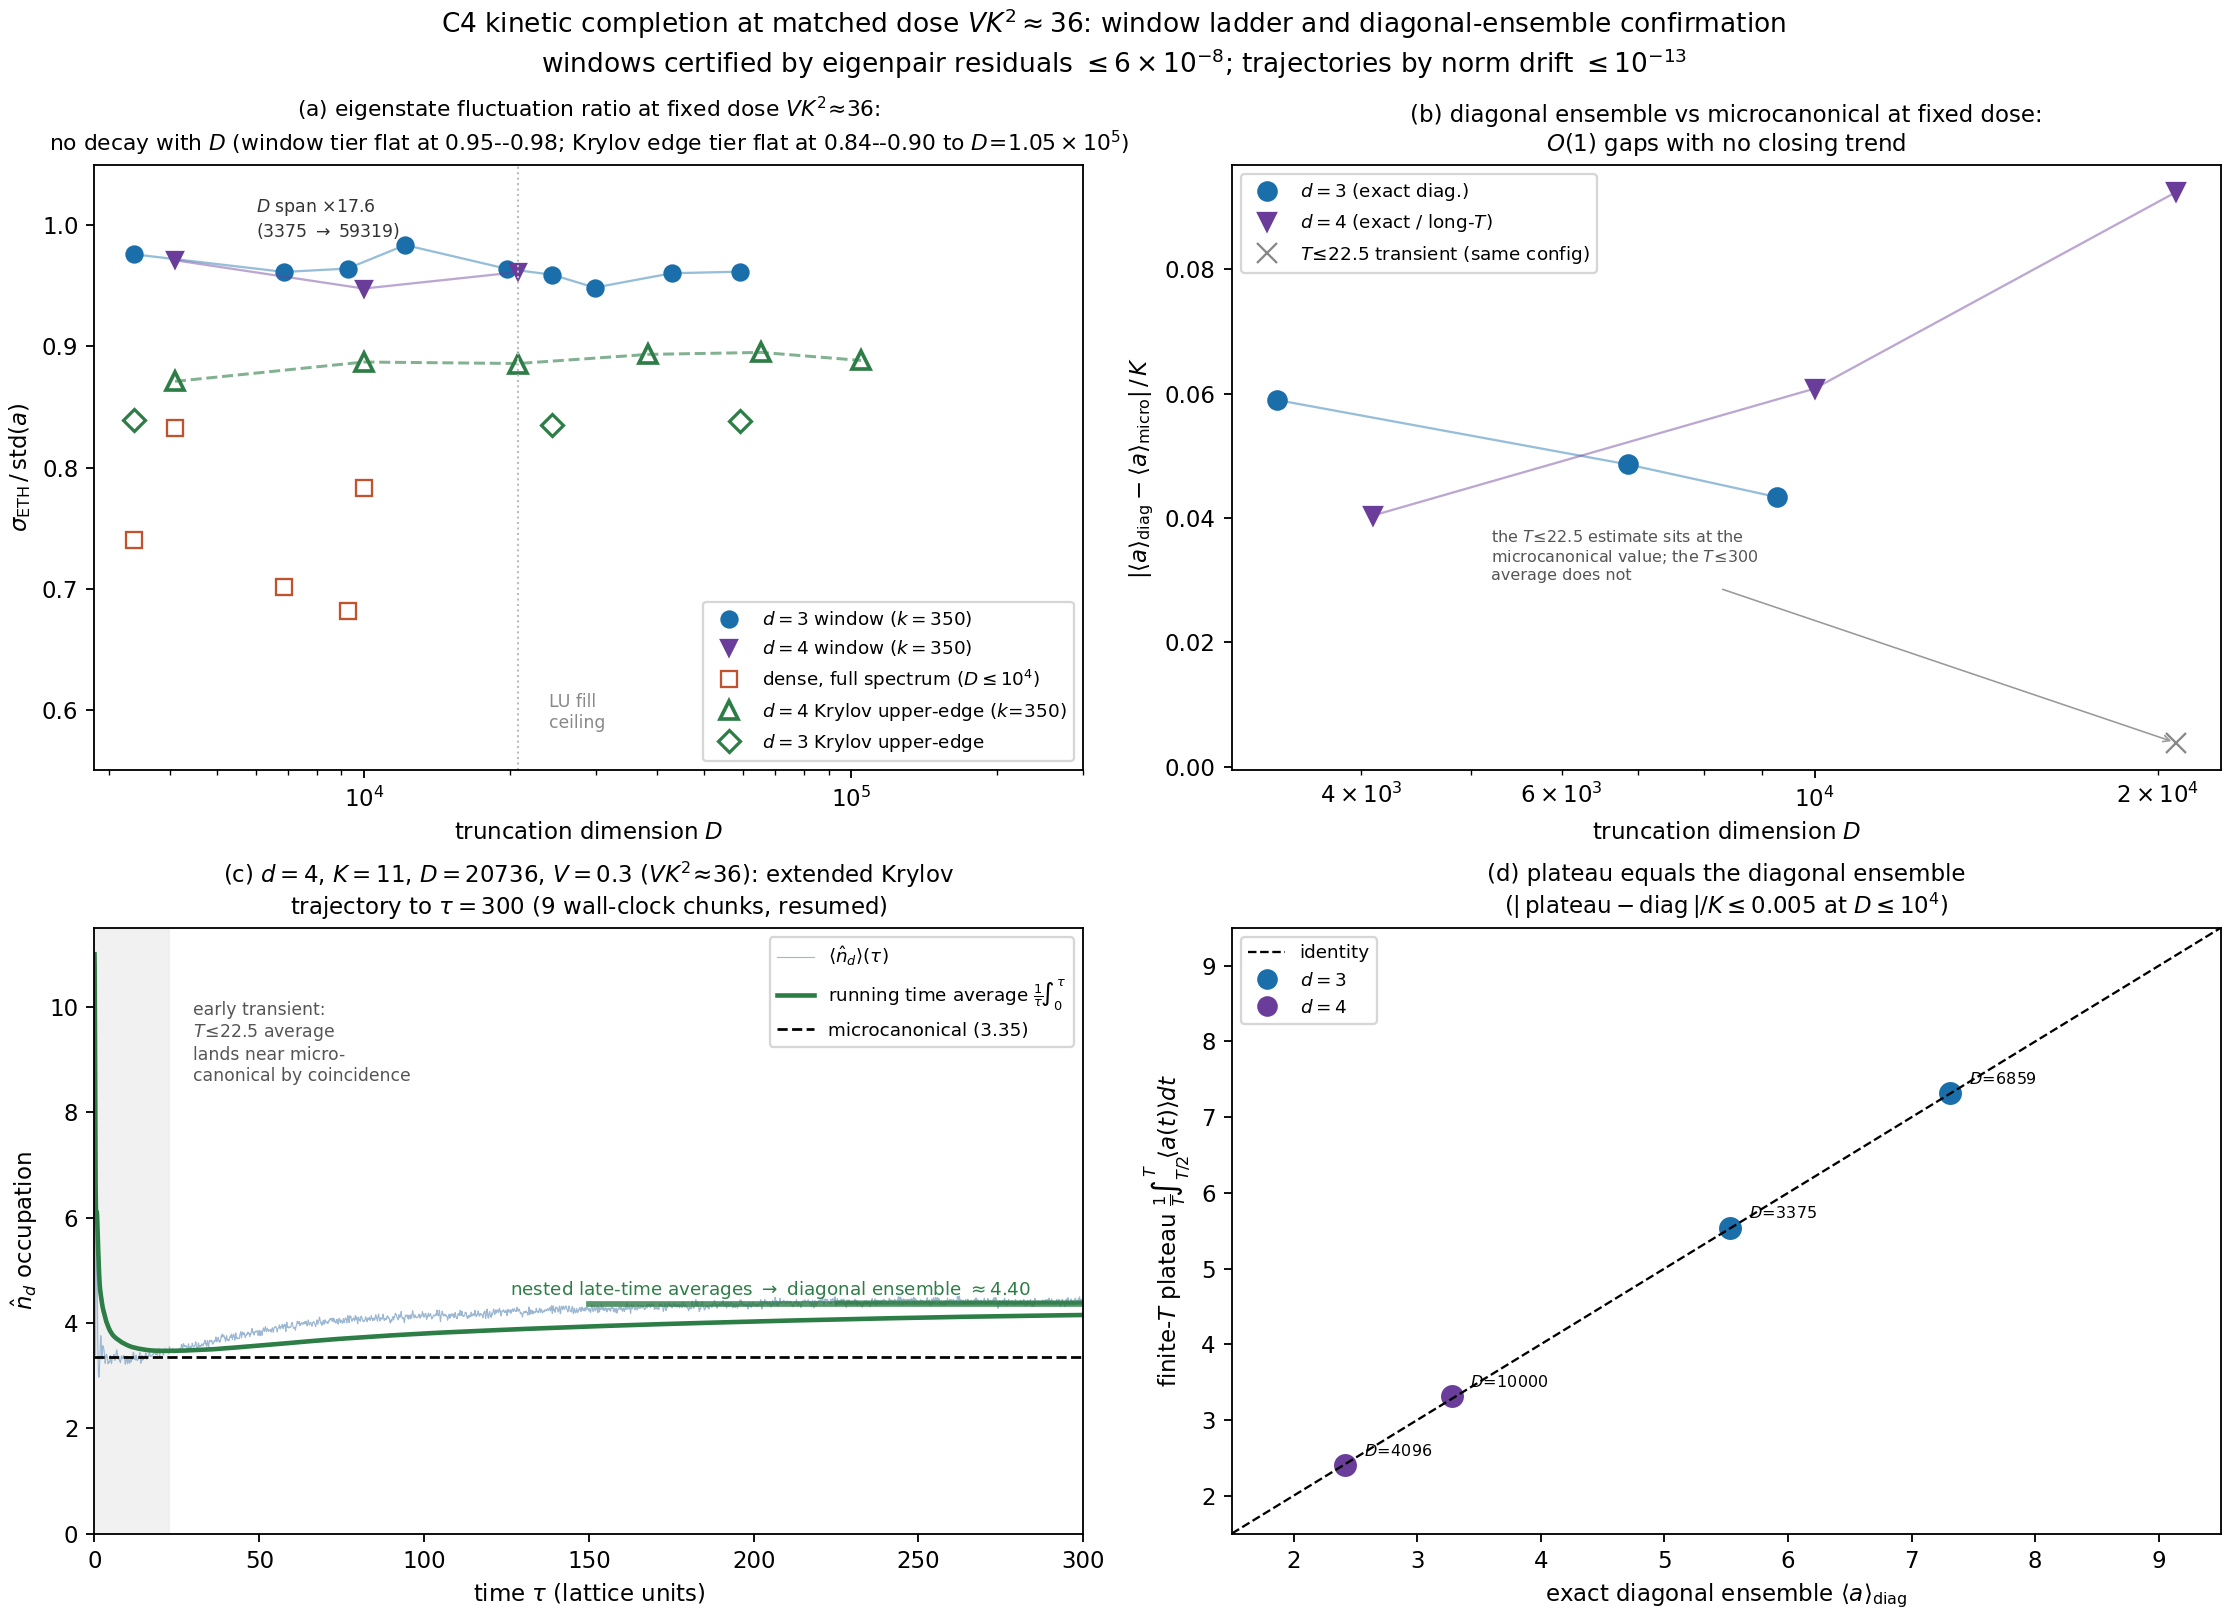
\includegraphics[width=\textwidth]{fig_c4_ladder.png}
\caption{Matched-dose ($VK^{2}\approx36$) numerics for the kinetic completion
(Remark~\ref{rem:numerics}(d)--(e)). (a)~Eigenstate fluctuation ratio
$\sigma_{\mathrm{ETH}}/\mathrm{std}(a)$ versus truncation dimension: window values
(filled) and exact full-spectrum values (open); no decay across a factor $17.6$ in $D$.
(b)~Distance of the diagonal ensemble from the microcanonical value, normalized by $K$:
$O(1)$ gaps with no closing trend; the $T\leq22.5$ estimate (cross) is a transient that
coincides with the microcanonical value. (c)~The $d=4$, $K=11$, $D=20736$, $V=0.3$
trajectory extended to $\tau=300$: observable, running time average, nested late-time
averages (diagonal-ensemble estimate $\approx4.40$), microcanonical line, and the early
transient. (d)~Finite-$T$ plateau versus exact diagonal ensemble at $D\leq10^{4}$ (identity
line).}
\label{fig:ladder}
\end{figure}

Falsifiers and test routes are listed in
Section~\ref{sec:register}.

\subsection{The Janus state}

A natural boundary condition is the vacuum: the claim that ``at the past hypothesis the
phase $1^{-i\omega_{0}\tau}=1$: time does not exist at $n=1$; time turns on when the universe
transitions to composite states.'' Under $H_{P}$ \emph{nothing} ever transitions
(Proposition~\ref{prop:frozen}), so the claim would be empty; under $H_{\mathrm{tot}}$ the vacuum
$\ket{1}$ is \emph{not} an eigenstate (because $H_{W}\ket{1}=\sum_{p}g_{p}\ket{p}$), and the
statement becomes substantive and true:

\begin{proposition}[Nucleation from the Janus state]\label{prop:nucleation}
For $H_{\mathrm{tot}}$ with $H_{W}\neq0$ and initial state $\psi(0)=\ket{1}$:
\begin{equation}
\psi(\tau)=\ket{1}-\frac{i\tau}{\hbar}\sum_{p\in P_{f}}g_{p}\ket{p}+O(\tau^{2}),
\end{equation}
so the \emph{total primon number} grows initially at rate
$d\langle\Nhat_{\mathrm{tot}}\rangle/d\tau=2\,\mathrm{Im}\,\langle\psi|H_{W}|\psi\rangle
/\hbar+O(\tau)=\frac{2\tau}{\hbar^{2}}\sum_{p}g_{p}^{2}+O(\tau^{2})>0$. The unique
zero-entropy state $\ket{1}$ is a regular point of the dynamics, not a fixed point; under
$H_{P}$ alone it is a fixed point (Proposition~\ref{prop:frozen}).
\end{proposition}

\begin{proof}
First-order time-dependent perturbation theory around the eigenstate $\ket{1}$ of $H_{P}$
(the Dyson series in $H_{W}+H_{\mathrm{hop}}$; $H_{\mathrm{hop}}$ annihilates the vacuum).
\end{proof}

Time, in this framework, is switched on by the interaction sector, with a mechanism that
exists. The stronger claims that
the actual history of the universe \emph{begins} at $\ket{1}$, and that the entropy profile is
two-sided (Janus-shaped) about that event, are boundary-condition statements and are demoted
to Conjectures $\mathsf{C7}$ and $\mathsf{C8}$; what remains as theorem is only the
uniqueness and zero entropy of the floor (Theorem~\ref{thm:spectrum} and
Section~\ref{sec:thermo}).

\section{Recurrence, Periodicity, and the Fate of Eternal Return}\label{sec:recurrence}

The anti-cyclical verdict---that prime arithmetic rigorously forbids exact cyclical
time and the universe cannot repeat---decomposes into a theorem, a correct application,
and two qualifications. This section separates them. The
resulting statement is \emph{stronger} than the slogan, because it identifies
exactly which recurrence phenomena are forbidden, which are unavoidable, and what the
boundary between them depends on.

\subsection{Linear independence of the prime logarithms}

\begin{lemma}[Fundamental-theorem independence]\label{lem:independence}
The set $\{\log p:p\in\Pr\}$ is $\Qq$-linearly independent. In particular, for distinct primes
$p,q$, the ratio $\log p/\log q$ is irrational.
\end{lemma}

\begin{proof}
Suppose $\sum_{i=1}^{r}q_{i}\log p_{i}=0$ with $q_{i}=a_{i}/b_{i}\in\Qq$ and distinct primes
$p_{i}$. Let $B=\mathrm{lcm}(b_{i})$ and $c_{i}=Bq_{i}\in\Zz$. Then
$0=\sum_{i}c_{i}\log p_{i}=\log\prod_{i}p_{i}^{c_{i}}$ (negative exponents handled by clearing
signs into the other side), so $\prod_{i}p_{i}^{c_{i}}=1$. Unique factorization forces
$c_{i}=0$ for all $i$, hence $q_{i}=0$.
\end{proof}

\subsection{Exact periodicity is forbidden}

\begin{theorem}[No exact return for generic states]\label{thm:noperiod}
Let $\psi=\sum_{n}c_{n}\ket{n}$ and let $S(\psi)=\{n:c_{n}\neq0\}$ be its support. The
following are equivalent:
\begin{enumerate}[leftmargin=1.6em]
\item There exists $\tau>0$ with $e^{-i\tau H_{P}/\hbar}\psi=\psi$;
\item There exists $T>0$ such that $\omega_{0}T\log n\in2\pi\Zz$ for every $n\in S(\psi)$;
\item The set $\{\log n:n\in S(\psi)\}$ is contained in $\alpha\,\Zz$ for some $\alpha>0$
(all supports are integer multiples of a common logarithmic unit; equivalently all $n\in
S(\psi)$ are powers of a single integer).
\end{enumerate}
In particular, if $S(\psi)$ contains any two integers $m,n$ that are not powers of a common
integer---for example any pair among $\{2,3\}$, $\{6,10\}$, $\{2,6\}$---then $\psi$ is
aperiodic: $e^{-i\tau H_{P}/\hbar}\psi\neq\psi$ for every $\tau>0$. The same holds for
$H_{\mathrm{tot}}$ whenever its spectrum is simple and contains two levels whose difference is
irrational in units of $\hbar/\omega_{0}$, which holds generically.
\end{theorem}

\begin{proof}
$e^{-i\tau H_{P}/\hbar}\psi=\sum_{n}c_{n}e^{-i\omega_{0}\tau\log n}\ket{n}$ equals $\psi$ iff
$e^{-i\omega_{0}\tau\log n}=1$ for all $n\in S(\psi)$, i.e. iff
$\omega_{0}\tau\log n\in2\pi\Zz$ for all such $n$. Setting $\alpha=2\pi/(\omega_{0}\tau)$,
this says every $\log n$ in the support lies in $\alpha\Zz$. If $m,n\in S$ and
$\log m,\log n\in\alpha\Zz$ with $\log m/\log n\notin\Qq$, the condition fails for every
$\tau$; by Lemma~\ref{lem:independence}, $\log 2/\log 3\notin\Qq$ etc.
\end{proof}

This is the rigorous core of the anti-cyclic verdict: \emph{eternal return in the exact sense
requires the support of the universal state to lie in a single geometric progression of
integers}, and no physically motivated state does.

\subsection{What is \emph{not} forbidden: three qualifications}

\begin{corollary}[Truncated systems recur]\label{cor:truncatedrecurrence}
Fix a finite truncation: primes $p\leq X$ and occupations $k_{p}\leq K$, so the Hilbert space
is finite-dimensional and the spectrum $\{E_{j}\}$ of $H_{P}$ (or of any self-adjoint
extension) is finite. Then the evolution $U(\tau)=e^{-i\tau H/\hbar}$ is a quasi-periodic
rotation, and for every state $\psi$ and every $\varepsilon>0$ the set
$\{\tau>0:\|U(\tau)\psi-\psi\|<\varepsilon\}$ is \emph{relatively dense} (there exists
$L=L(\varepsilon,\psi)$ such that every interval of length $L$ contains such a $\tau$). In
particular Poincar\'e recurrence holds in its strongest (uniform, Bohr almost-periodic) form.
This is the finite-dimensional special case of Theorem~\ref{cor:nopoincare} below, recorded
separately because it is the form in which recurrence appears in any \emph{computation}.
\end{corollary}

\begin{proof}
On a finite-dimensional space $U(\tau)=e^{-i\tau\Lambda}$ with
$\Lambda=\mathrm{diag}(E_{1},\dots,E_{d})/\hbar$; the map $\tau\mapsto
(e^{-i\tau E_{1}/\hbar},\dots,e^{-i\tau E_{d}/\hbar})$ is a continuous one-parameter
subgroup of the compact torus $\mathbb{T}^{d}$, and every orbit of a compact group rotation is
uniformly recurrent: the return times to any neighborhood of the identity are syndetic. This
is Kronecker's theorem in its group form \cite{hardywright2008}.
\end{proof}

\begin{theorem}[Uniform recurrence of the free flow, infinite system]\label{cor:nopoincare}
For \emph{every} state $\psi\in\Hil_{\mathcal{A}}$ and every $\varepsilon>0$, the set of
$\varepsilon$-return times
\begin{equation}
\Bigl\{\tau>0:\ \bigl\|e^{-i\tau H_{P}/\hbar}\psi-\psi\bigr\|<\varepsilon\Bigr\}
\end{equation}
is \emph{relatively dense} in $\Rr$. The free arithmetic flow is Bohr almost periodic for
all states, with no finite invariant measure required and no truncation assumed. What fails
is not $\varepsilon$-recurrence but its \emph{uniformity in the state}: the return-time
scale $L(\varepsilon,\psi)$ is unbounded as a function of $\psi$ (it grows with the
Diophantine complexity of the finite supports approximating $\psi$), and exact return
remains forbidden by Theorem~\ref{thm:noperiod}.
\end{theorem}

\begin{proof}
Fix $\varepsilon>0$ and $\psi=\sum_{n}c_{n}\ket{n}\in\ell^{2}$. Choose a finite support set
$F\subset\Nn_{\geq1}$ with $\sum_{n\notin F}|c_{n}|^{2}<\varepsilon^{2}/4$. The truncated
flow $\tau\mapsto\bigl(e^{-i\omega_{0}\tau\log n}\bigr)_{n\in F}$ is a continuous
one-parameter subgroup $h\colon\Rr\to\mathbb{T}^{F}$; let
$H=\overline{h(\Rr)}$, a compact connected subgroup of the torus. The $\Rr$-orbit of the
identity under left translation by $h(\tau)$ is dense in $H$ by construction, and a dense
orbit of an equicontinuous (group) action on a compact space is minimal; minimal
equicontinuous flows are uniformly recurrent, so
$T(\delta)=\{\tau:d(h(\tau),e_{H})<\delta\}$ is relatively dense for every $\delta>0$.
Taking $\delta$ small enough that all phases on $F$ deviate by less than $\varepsilon/2$
in the $\ell^{2}$ sense (finitely many constraints), we obtain
$\|U(\tau)\psi-\psi\|\leq\varepsilon/2+\varepsilon/2$ for every $\tau\in T(\delta)$, a
relatively dense set. The non-uniformity in $\psi$ follows because $F$ must grow as the
tails of $\psi$ shrink, and the Diophantine return times on $F$ are unbounded in $|F|$ (for
supports with rationally independent generators, Kronecker's theorem gives relative density
but no uniform bound: the minimal return time for $F=\{2,3,\dots,p_{|F|}\}$ grows at least
exponentially in $|F|$, since the frequencies $\log n$ are rationally independent by
Lemma~\ref{lem:independence} and simultaneous approximation of independent frequencies is
slow).
\end{proof}

The third qualification concerns the \emph{classical} multiplicative walk, and it sharpens
the boundary of the no-cycle verdict in an unexpected direction.

\begin{proposition}[P\'olya transience of the multiplicative walk]\label{prop:polya}
Consider the classical random walk on the divisibility graph of
Definition~\ref{def:multiplication} restricted to $d=|P_{f}|$ active primes: from
$k=(k_{1},\dots,k_{d})\in\Zz_{\geq0}^{d}$ step to $k+e_{j}$ with probability $1/(2d)$ and to
$k-e_{j}$ (when $k_{j}>0$) with probability $1/(2d)$, staying otherwise. Then the walk is
recurrent for $d\leq2$ and transient for $d\geq3$ \cite{polya1921}. In particular for
$d\geq3$ the walk returns to the vacuum $k=0$ (the Janus state) only finitely many times,
almost surely.
\end{proposition}

Proposition~\ref{prop:polya} has a striking interpretive reading: whether
the arithmetic universe ``cycles back to its origin'' depends on the \emph{number of active
prime modes}. With one or two primes, the multiplicative universe is recurrent---a rigorous
echo of cyclical cosmology. With three or more, it is transient, and the Janus point is a
genuinely singular origin. The absolute prohibition thus becomes a structural,
checkable dichotomy.

\subsection{The verdict on cyclical time}

Assembling the three legs: exact eternal return is impossible for states whose support spans
incommensurable integers (Theorem~\ref{thm:noperiod}); $\varepsilon$-approximate recurrence is
universal for the \emph{free} flow, at every state, with return times relatively dense but
astronomically non-uniform (Theorem~\ref{cor:nopoincare}, and
Corollary~\ref{cor:truncatedrecurrence} for the trivial finite case); and the \emph{cascading}
(or classical walk) dynamics is transient for $d\geq3$ modes (Proposition~\ref{prop:polya}),
with the interacting quantum system conjecturally non-recurrent on every physical scale
(Conjecture $\mathsf{C4}$). The philosophical consequences
are drawn in Section~\ref{sec:philosophy}; the essential point is that the framework's
anti-cyclical verdict survives as a \emph{layered} statement---exact return forbidden as a
genuine theorem, practical return driven out of reach by Diophantine slowness, transience
of the cascade for three or more active modes---rather than as an absolute metaphysical
prohibition. The free arithmetic sector, left to itself, is the \emph{most} recurrent object
in the theory (Bohr almost periodicity for all states, Theorem~\ref{cor:nopoincare}); all
irreversibility is therefore manufactured by the interaction sector and the boundary
condition, never by the spectrum. This is the sharpest available form of the intuition
that ``the river never circles back,'' and it is also the form most useful to
the arrow-of-time analysis of Sections~\ref{sec:time} and~\ref{sec:philosophy}.

% =====================================================================
% SECTION 5: The arithmetic clock  +  SECTION 6: Thermodynamics & gravity
% =====================================================================

\section{The Arithmetic Clock and the Problem of Time}\label{sec:time}

\subsection{The problem of time, stated precisely}

The reconciliation problem for the two classical concepts of time is standard: in
quantum mechanics, $t$ is an external parameter and the Schr{\"o}dinger equation evolves
states with respect to it; in general relativity, elapsed time is the proper time along a
worldline, $\tau_{\gamma}=c^{-1}\int_{\gamma}\sqrt{-g_{\mu\nu}dx^{\mu}dx^{\nu}}$, a geometric
quantity that varies from trajectory to trajectory, while the canonical Hamiltonian of
gravity is a constraint, $\Hmax\Psi=0$, with no external evolution at all. The
resolution is relational: time is a correlation between subsystems, realized quantum
mechanically by the Page--Wootters mechanism \cite{pagewootters1983}, with the primon
spectrum supplying the clock. This section turns that resolution into theorems, corrects
one sign-of-life issue (the clock kernel never decorrelates, so the arrow
of time cannot live in the clock), and quantifies the claim that ``at the
Janus point time does not exist.''

The Page--Wootters construction is standard: for a total state $\Psi$ satisfying a constraint
$(H_{C}+H_{S})\Psi=0$ of clock-plus-system, the conditional state of the system when the
clock reads $\tau$ is $\psi_{S}(\tau)=\bra{\tau}\Psi\rangle$, and for an ideal clock family
this satisfies an effective Schr{\"o}dinger equation in $\tau$. All content therefore
concentrates in the clock family. The analysis below supplies the \emph{kinematical} level of
this program: the clock family, the conditional-state map, and the correlation kernel. The
constraint equation itself is not solved here---solving it requires the interaction sector of
Section~\ref{sec:dynamics} and belongs to the content of $\mathsf{C4}$---and no claim is made
that this section dissolves the problem of time; what is proved is the exact correlation
structure of the arithmetic clock, and the exact statement of what that structure forbids.

\subsection{The zeta clock}

\begin{definition}[Zeta clock family]\label{def:clock}
For a dimensionless regulator $\nu>\tfrac12$ define the normalized clock states
\begin{equation}\label{eq:clockstates}
\ket{\tau;\nu}\;=\;\zeta(2\nu)^{-1/2}\sum_{n=1}^{\infty}n^{-\nu-i\omega_{0}\tau}\ket{n},
\end{equation}
a unit-norm family in $\Hil_{\mathcal{A}}$ (unit norm because $\sum_{n}n^{-2\nu}=\zeta(2\nu)$
converges for $2\nu>1$). The regulator is a resolution parameter, not a temperature: the
weights $n^{-\nu}$ confine the clock to energies of order
$\hbar\omega_{0}/(2\nu-1)$, as computed in Proposition~\ref{prop:uncertainty}. A clock at
regulator $\nu$ has the same mean energy as a canonical primon state at $\sigma=2\nu$; the
clock family therefore exists on \emph{both} sides of the Hagedorn scale---$\nu\downarrow\tfrac12$
is the high-energy (canonical-divergence) limit, $\nu\to\infty$ the vacuum limit---and it is
the analytic object through which energies above $T_{H}$, where no Gibbs state exists, are
nevertheless resolved (Section~\ref{sec:arithmetic}).
\end{definition}

\begin{proposition}[Clock covariance and two-time kernel]\label{prop:kernel}
\begin{enumerate}[leftmargin=1.6em]
\item (Covariance.) $e^{-i\tau' H_{P}/\hbar}\ket{\tau;\nu}=\ket{\tau+\tau';\nu}$: clock
translations are generated by $H_{P}$ itself, so the clock reading $\tau$ is exactly the
phase parameter conjugate to $\log\Nhat$,
\begin{equation}
e^{-i\omega_{0}\tau\log\Nhat}\ket{n}=n^{-i\omega_{0}\tau}\ket{n}.
\end{equation}
\item (Two-time kernel.) For all $\tau,\tau'$,
\begin{equation}\label{eq:kernel}
\braket{\tau';\nu}{\tau;\nu}
\;=\;\frac{\zeta\bigl(2\nu-i\omega_{0}(\tau-\tau')\bigr)}{\zeta(2\nu)}.
\end{equation}
\item (Positivity.) The kernel \eqref{eq:kernel} is positive definite on $\Rr$: it is the
Fourier transform of the probability measure
$\mu_{\nu}=\zeta(2\nu)^{-1}\sum_{n}n^{-2\nu}\delta_{\log n}$ on the energy-per-mode
variable $u=\log n$.
\item (Product of phases.) For a superposition $\sum_{n}c_{n}\ket{n}$ evolved for time
$\tau$, the phase acquired is $n^{-i\omega_{0}\tau}$, and by unique factorization
\begin{equation}
n^{-i\omega_{0}\tau}=\prod_{p}p^{-i\omega_{0}\tau\,k_{p}}:
\end{equation}
each prime contributes an elementary phase generator, and composite evolution is the product
of prime evolutions. This is the exact sense in which ``primes provide the elementary
generators of spectral phase order.''
\end{enumerate}
\end{proposition}

\begin{proof}
(1) is immediate term by term. (2) $\braket{\tau';\nu}{\tau;\nu}
=\zeta(2\nu)^{-1}\sum_{n}n^{-2\nu}e^{i\omega_{0}(\tau-\tau')\log n}
=\zeta(2\nu)^{-1}\zeta(2\nu-i\omega_{0}(\tau-\tau'))$, since
$e^{i\omega_{0}\Delta\tau\log n}=n^{i\omega_{0}\Delta\tau}$. (3) The kernel
$K(\Delta\tau)=\int e^{i\omega_{0}\Delta\tau u}\,d\mu_{\nu}(u)$ is the characteristic
function of $\mu_{\nu}$ composed with a dilation, hence positive definite by Bochner's
theorem. (4) follows from unique factorization applied to the logarithm of the phase.
\end{proof}

Equation~\eqref{eq:kernel} is the framework's signature formula: \emph{the
distinguishability of two readings of the arithmetic clock is governed by the Riemann zeta
function}. What follows adds
the facts that make it usable.

\begin{theorem}[Almost-periodicity of the clock: the arrow cannot live here]\label{thm:bohr}
For every $\nu>\tfrac12$, the kernel $K(\Delta\tau)=\zeta(2\nu-i\omega_{0}\Delta\tau)/\zeta(2\nu)$
is a Bohr almost-periodic function of $\Delta\tau$ \cite{besicovitch1932} (the Dirichlet series
converges absolutely on the line $\sigma=2\nu>1$). Consequently:
\begin{enumerate}[leftmargin=1.6em]
\item $|K|$ does \emph{not} decay along any sequence: $\limsup_{|\Delta\tau|\to\infty}|K(\Delta\tau)|=1$.
\item For every $\varepsilon>0$ the set
$\{\Delta\tau:|K(\Delta\tau)-1|<\varepsilon\}$ is relatively dense: clock correlations
resynchronize infinitely often, in both time directions, at every resolution $\nu$.
\end{enumerate}
No limit $\nu\downarrow\tfrac12$ escapes this: at every fixed $\nu$ the kernel is two-sided
symmetric, and the singular limit only narrows the correlation peak
(Proposition~\ref{prop:uncertainty}(2)) without ever selecting a direction. The high-energy
clock is \emph{more} resolved, not \emph{directed}.
\end{theorem}

\begin{proof}
On the line $\sigma=2\nu>1$, $\zeta(s)=\sum_{n}n^{-s}$ is an absolutely convergent Dirichlet
series with $\sum_{n}n^{-\sigma}<\infty$, hence a (uniform limit of finite exponential sums)
Bohr almost-periodic function of the imaginary part \cite{besicovitch1932}. Almost-periodic
functions have relatively dense $\varepsilon$-almost-periods, and $K(0)=1$.
\end{proof}

This theorem resolves a hidden tension in the framework. The zeta
object appears twice: as the clock (``the distinguishability of two times is
governed by the zeta function'') and as the engine of the thermodynamic arrow (``the
cascade up the mountain of composite numbers''). Theorem~\ref{thm:bohr} shows
these two roles cannot be fused: an almost-periodic clock is \emph{recurrent} and carries no
arrow. In the framework the arrow is therefore relocated entirely to the
interaction sector and the boundary condition (Conjecture $\mathsf{C4}$ and $\mathsf{C7}$),
while the clock contributes the neutral, arrow-free, maximally stable phase reference. This
is a structural clarification, not a loss: it says that \emph{within the framework, time
measurement and time's arrow are functionally separated objects}, exactly as relational
philosophy of time requires.

\subsection{Energy--time duality of the arithmetic clock}

\begin{proposition}[Resolution duality]\label{prop:uncertainty}
For the clock family $\ket{\tau;\nu}$:
\begin{enumerate}[leftmargin=1.6em]
\item The mean energy is
$\langle H_{P}\rangle_{\nu}=\hbar\omega_{0}\bigl(-\zeta'/\zeta\bigr)(2\nu)
=\dfrac{\hbar\omega_{0}}{2\nu-1}+O(\hbar\omega_{0})$ as $\nu\downarrow\tfrac12$.
\item The correlation peak is asymptotically Lorentzian: as $\nu\downarrow\tfrac12$,
uniformly for bounded $\omega_{0}\Delta\tau/(2\nu-1)$,
\begin{equation}
|K(\Delta\tau)|^{2}
=\frac{(2\nu-1)^{2}}{(2\nu-1)^{2}+\omega_{0}^{2}\Delta\tau^{2}}\,\bigl(1+o(1)\bigr),
\end{equation}
with half-width $\Delta\tau_{1/2}\asymp(2\nu-1)/\omega_{0}$.
\item Consequently $\langle H_{P}\rangle_{\nu}\,\Delta\tau_{1/2}\to\hbar$ as
$\nu\downarrow\tfrac12$: the zeta clock asymptotically saturates the
Mandelstam--Tamm energy--time limit. Time resolution is bought one-for-one with clock energy,
and the clock never becomes ``cheap.''
\item Conversely, as $\nu\to\infty$ the state concentrates on $\ket{1}$:
$\ket{\tau;\nu}\to\ket{1}$, energy $\to0$, and $K\to1$ for all $\Delta\tau$: the clock
resolves nothing. At the Janus limit the clock degenerates---the quantified form of the
claim that ``at $n=1$ time does not exist.''
\end{enumerate}
\end{proposition}

\begin{proof}
(1) is Theorem~\ref{thm:hagedorn} at $\sigma=2\nu\downarrow1$. Positivity of $\langle H_P\rangle$ requires $\nu>1/2$, consistent with Definition~\ref{def:clock}. (2) Near the pole,
$\zeta(\sigma-it)=(\sigma-1-it)^{-1}+O(1)$, so
$|K|^{2}=|\sigma-1|^{2}/((\sigma-1)^{2}+t^{2})+o(1)$ with $t=\omega_{0}\Delta\tau$ and
$\sigma-1=2\nu-1$. (3) Multiply (1) and (2). (4) $n^{-2\nu}$ concentrates on $n=1$;
$K(t)=\zeta(2\nu-it)/\zeta(2\nu)\to1$ since $\zeta(2\nu-it)\to1$ and
$\zeta(2\nu)\to1$.
\end{proof}

\subsection{Reconciliation of the three times}

With the clock machinery in place, the tripartite reconciliation can be stated as
a compact conditional statement. \emph{Quantum-mechanical time} is the reading of a
relational clock in the classical-clock limit: it is recovered when the clock subsystem is
large, weakly coupled, and quasi-classical, in which case $\tau_{\mathrm{clock}}\approx t$
for all practical observers. \emph{Relativistic time} is the proper-time functional along
worldlines: it is the geometric content of the clock's embedding, determining which phase
increments accumulate along which trajectory. \emph{Quantum-gravitational time} is the
constraint-generated phase correlation: with the primon clock, $\tau$ is conjugate to
$\log\Nhat$, and evolution is the multiplicative phase flow
$n^{-i\omega_{0}\tau}$. The three are not rivals but levels: the block-level correlation
structure ($\Hmax\Psi=0$), its geometric projection (proper time), and its semiclassical
limit (external $t$). All incompatibilities of principle dissolve at the kinematical level;
what remains open
is whether the \emph{specific} identification of the clock with the
primon spectrum is realized (Conjecture $\mathsf{C1}$), and how the geometric sector
emerges from the arithmetic one (Conjectures $\mathsf{C3}$, $\mathsf{C9}$).

The tripartite reconciliation is compactly stated:
\begin{center}
\emph{Relativity provides the geometry; quantum mechanics provides the spectrum; the primes
provide the arithmetic order of the spectrum; and time is the phase relation among
prime-ordered states measured along geometric worldlines.}
\end{center}
The measurement clause is Proposition~\ref{prop:kernel}(1) (clock covariance); the ordering
clause is unique factorization, i.e. Proposition~\ref{prop:kernel}(4); the arrow clause is
conspicuously absent, by Theorem~\ref{thm:bohr}, and lives in the interaction sector.

\section{Thermodynamics, Gravity, and the Holographic Bridge}\label{sec:thermo}

\subsection{The exact counting law}

A repeatedly used statement is ``the number of states below energy $E$ grows like
$e^{E/\hbar\omega_{0}}$.'' The exact statement is a one-line identity, and its precision is
what makes the holographic bridge in Section~\ref{sec:holography} clean.

\begin{theorem}[Log-count identity]\label{thm:logcount}
Let $N(E)=\#\{n\in\Nn_{\geq1}:\hbar\omega_{0}\log n\leq E\}=\lfloor e^{E/\hbar\omega_{0}}\rfloor$,
and write $x=E/\hbar\omega_{0}$ and $r(E)=\log N(E)-x$. Then:
\begin{enumerate}[leftmargin=1.6em]
\item (Global envelope.) For all $E\geq0$: $-\log2\leq r(E)\leq0$.
\item (Sharp two-sided bound, $E\geq\hbar\omega_{0}\log2$.)
\begin{equation}\label{eq:sharpdefect}
\log\bigl(1-e^{-x}\bigr)\;\leq\; r(E)\;\leq\; 0,
\end{equation}
with both bounds sharp: $r\uparrow0$ as $E$ crosses a level from above, and
$r\downarrow\log(1-e^{-x})$ as $E$ approaches a level from below.
\item (Exponential decay.) $|r(E)|\leq-\log(1-e^{-x})\leq 2e^{-x}$: the defect converges to
zero \emph{exponentially}. The counting function itself remains a staircase forever: $N$
jumps by one at every level $E=\hbar\omega_{0}\log m$, and the jump of $\log N$ there is
$\log\bigl(1+\tfrac1m\bigr)\sim\tfrac1m$---the granularity persists at every scale while its
amplitude decays like $e^{-x}$.
\item (Smoothing.) For every probability kernel $w$ supported in $[-\Delta,\Delta]$ with
$\Delta$ fixed, the smoothed count $\widetilde N=N\ast w$ satisfies, uniformly in
$E\geq\hbar\omega_{0}(\log2+\Delta)$,
\begin{equation}\label{eq:smoothing}
\log\widetilde N(E)\;=\;x\;+\;\log\!\int e^{t}w(t)\,dt\;+\;O(e^{-x}):
\end{equation}
the growth rate of every fixed-window smoothing of the entropy is exactly $1/\hbar\omega_{0}$
up to exponentially small corrections, at every energy scale.
\end{enumerate}
In particular the microcanonical entropy $S(E)=k_{B}\log N(E)$ satisfies
\begin{equation}
S(E)\;=\;\frac{E}{T_{H}}\;+\;\delta(E),
\qquad
|\delta(E)|\;\leq\;k_{B}\log\frac{1}{1-e^{-E/\hbar\omega_{0}}}\;\leq\;2k_{B}e^{-E/\hbar\omega_{0}}
\quad(E\geq\hbar\omega_{0}\log2),
\end{equation}
with $T_{H}=\hbar\omega_{0}/k_{B}$. (The unsmoothed entropy is a staircase; its pointwise
microcanonical temperature is undefined between levels. The content of the Hagedorn reading
is item~(iv): the growth rate is energy-independent, so energy input converts into state
multiplicity at a fixed exchange rate.)
\end{theorem}

\begin{proof}
$N(E)=\lfloor e^{x}\rfloor$ because $\hbar\omega_{0}\log n\leq E\iff n\leq e^{x}$. Write
$y=e^{x}$ and $\{y\}=y-\lfloor y\rfloor\in[0,1)$, so $r=\log\bigl(1-\{y\}/y\bigr)\in[\log(1-1/y),0]$
since $\lfloor y\rfloor\geq y-1$ and $\{y\}<1$. The lower bound is approached as $\{y\}\uparrow1$
($E$ approaching a level from below), the upper bound attained as $\{y\}\downarrow0$. Decay:
$-\log(1-u)\leq2u$ for $u\leq\tfrac12$, and $\{y\}/y<1/y=e^{-x}\leq\tfrac12$ for $x\geq\log2$.
Jumps: on $y\in[m,m+1)$, $\log N=\log m$ and the jump at $y=m+1$ is
$\log\bigl((m+1)/m\bigr)\sim1/m$. Smoothing: $N(E+t)=e^{x+t}-\{e^{x+t}\}$, so
$\widetilde N(E)=e^{x}\int e^{t}w(t)\,dt-R(E)$ with $0\leq R(E)=\int w(t)\{e^{x+t}\}\,dt\leq1$;
hence $\log\widetilde N=x+\log\int e^{t}w(t)dt+\log\bigl(1-R(E)e^{-x}/\!\int e^{t}w\bigr)$ and
the last term is $O(e^{-x})$, uniformly in $E$.
\end{proof}

Two consequences of the corrected defect estimate are load-bearing later, and both follow
from item~(iii). First, at matched entropy scale the integer-counting fluctuation is
$O(k_{B}e^{-E/\hbar\omega_{0}})$: \emph{far smaller} than the logarithmic corrections of
black-hole entropy, so those corrections cannot originate from the floor sector at
all---Section~\ref{sec:holography} turns this from a caveat into a falsifier (the counting
contributes no $\log A$ term; any such term must be carried by the dictionary). Second, the
fluctuation sector of the gravitational counting function is carried not by the floor but by
the \emph{prime}-counting oscillations: the explicit formula
$\psi(x)=x-\sum_{\rho}x^{\rho}/\rho+\cdots$ has fluctuations bounded by $O(\sqrt x\log^{2}x)$
under the Riemann hypothesis---the content of von Koch's equivalence
\cite{vonkoch1901}: the Riemann hypothesis is \emph{equivalent} to the statement that
arithmetic fluctuations about the smooth classical term are as small as
square-root-small. Read in the framework's dictionary, RH becomes: \emph{quantum
fluctuations of the arithmetic sector about the classical continuum are optimally
suppressed}. That is a rigorous reformulation of ``RH = spectral
stability'', and it is the strongest form of that claim that mathematics currently
licenses.

\subsection{The holographic bridge}\label{sec:holography}

The derivation of the Bekenstein--Hawking entropy from prime state counting
is a natural target. This paper isolates exactly one
nontrivial input and shows the rest is Theorem~\ref{thm:logcount}.

\begin{conjecture}[Arithmetic holographic bound]\label{conj:holobound}
The maximal primon excitation energy accessible in, or associated with, a spacetime region
whose boundary has area $A$ is
\begin{equation}\label{eq:holobound}
E_{\max}(A)\;=\;\frac{\hbar\omega_{0}}{4\ell_{P}^{2}}\,A\;+\;\hbar\omega_{0}\,s(A),
\qquad
s(A)=O\!\Bigl(\log\frac{A}{\ell_{P}^{2}}\Bigr),
\end{equation}
independently of the detailed matter content, where
$\ell_{P}=\sqrt{G\hbar/c^{3}}$ is the Planck length. The term $\hbar\omega_{0}s(A)$ is the
\emph{dictionary error term}: it is the only slot through which logarithmic corrections can
enter, since the counting theorem contributes none (Theorem~\ref{thm:logcount}(iii)).
\end{conjecture}

\begin{theorem}[Conditional Bekenstein--Hawking]\label{thm:bh}
Assume Conjecture~\ref{conj:holobound}. Then the arithmetic entropy of the region is
\begin{equation}
S(A)\;=\;k_{B}\log N\bigl(E_{\max}(A)\bigr)
\;=\;\frac{k_{B}A}{4\ell_{P}^{2}}\;+\;k_{B}\,s(A)\;+\;\delta\bigl(E_{\max}(A)\bigr),
\qquad
|\delta|\leq2k_{B}e^{-E_{\max}/\hbar\omega_{0}},
\end{equation}
which is the Bekenstein--Hawking entropy \cite{bekenstein1973,hawking1975} with the area
coefficient exact and \emph{every} logarithmic correction carried by the dictionary term
$s(A)$ and none by the counting. The pure model ($s=O(1)$) predicts no
$-\alpha\log(A/\ell_{P}^{2})$ term at all; a computed correction of that class (several
ensembles give $-\tfrac32\log A$) therefore falsifies the pure form and measures $s$.
Moreover, for a Schwarzschild black hole of
mass $M$, $A=16\pi G^{2}M^{2}/c^{4}$ and $A/4\ell_{P}^{2}=4\pi GM^{2}/(\hbar c)$; the choice
$E_{\max}=Mc^{2}$ and $\hbar\omega_{0}=2\,k_{B}T_{H}^{\mathrm{BH}}$ normalizes
\eqref{eq:holobound} \emph{exactly} at fixed horizon, with $T_{H}^{\mathrm{BH}}=\hbar c^{3}/(8\pi GMk_{B})$
the Hawking temperature.
\end{theorem}

\begin{proof}
Substitute \eqref{eq:holobound} into Theorem~\ref{thm:logcount}. For the Schwarzschild case,
$E_{\max}(A)/\hbar\omega_{0}=A/4\ell_{P}^{2}$ by \eqref{eq:holobound}; with
$E_{\max}=Mc^{2}$ this forces $\hbar\omega_{0}=4Mc^{2}\ell_{P}^{2}/A
=4Mc^{2}\cdot(G\hbar/c^{3})/(16\pi G^{2}M^{2}/c^{4})
=\hbar c^{3}/(4\pi GM)=2k_{B}T_{H}^{\mathrm{BH}}$.
\end{proof}

Two remarks delimit the bridge; both are registered under $\mathsf{C3}$.

\begin{remark}[The factor-of-two ambiguity]
The Hawking identification above is exact only per-horizon: since $T_{H}^{\mathrm{BH}}\propto
M^{-1}$, a \emph{universal} $\omega_{0}$ cannot equal $2T_{H}^{\mathrm{BH}}$ for all masses.
Either $\omega_{0}$ is universal and the identification holds to within
$O(1)$ horizon-dependent factors, or the arithmetic scale is set per horizon. Which
alternative survives is a genuine open question that the conjecture form makes explicit;
a presentation that silently treats $\omega_{0}$ as universal and the
identification as exact would hide it. In both alternatives the \emph{area coefficient} is
exact, because the counting defect is exponentially small (Theorem~\ref{thm:logcount}(iii));
all residual freedom lives in the dictionary term $s(A)$.
\end{remark}

\begin{remark}[What the bridge does and does not derive]
The bridge converts an area law into an \emph{energy} cutoff statement plus an exact
counting theorem; it does not derive the cutoff. This is precisely the logical position of
the holographic principle in mainstream theory, translated into arithmetic terms. The
conversion loss is provably zero in the area coefficient (Theorem
\ref{thm:logcount} has no hidden degeneracy factors, since the primon spectrum is simple,
Theorem~\ref{thm:spectrum}), and every logarithmic correction is imported through the
dictionary term $s(A)$: any slack in Conjecture~\ref{conj:holobound} is slack in the
physics, not in the counting.
\end{remark}

\subsection{Singularities and the Hagedorn wall}

The singularity claims swing between two poles: one places the primon gas
\emph{at} the singularity (the reported conformal system near the black-hole center), later
reading declares that singularities \emph{do not exist}. The reconciliation is a standard
move of effective field theory, and it is worth stating once, cleanly, because it removes
the apparent contradiction:

\begin{remark}[Resolution of the singularity tension]\label{rem:singularity}
``Singularity'' denotes the boundary of validity of the continuum effective description, not
a locus in the fundamental theory. In the reconstructed framework: the geometric (Einstein)
description fails where its implicit continuum counting diverges; the arithmetic description
remains finite at all energies (Theorem~\ref{thm:spectrum} has no finite accumulation
point, and all quantities are finite below $T_{H}$). The pole of $\zeta$ at $s=1$ is the
exact analytic signature of the breakdown: it is a \emph{critical} (Hagedorn) divergence,
not a curvature divergence. What the Big Bang and black-hole interiors ``are'' in this
framework is the regime where the geometric effective theory must be replaced by the
arithmetic one; the primon gas is the UV-complete description of \emph{that regime}, which is
compatible with it also being located, in the geometric coordinates of the effective theory,
``near the singularity.'' Both readings are thereby retained, each in its
proper tense. The associated physical conjecture ($\mathsf{C6}$) is that the Hagedorn wall
$T_{H}$ replaces the singular point: approach to the singularity is approach to a critical
temperature at which energy converts into primon creation rather than curvature growth.
\end{remark}

\subsection{Emergent gravity and the hierarchy problem}

The resolution of the hierarchy problem---gravity as an entropic, $1/N$-suppressed
collective effect \cite{jacobson1995,verlinde2011,thooft1974}---is the most speculative of
its physics claims, and it is demoted in full. But the demoted form can be made
unusually concrete, because the arithmetic sector supplies an explicit $N$.

\begin{conjecture}[Arithmetic hierarchy]\label{conj:hierarchy}
The Newton constant is set by the number of arithmetic degrees of freedom below the
effective cutoff $E_{\mathrm{cut}}$:
\begin{equation}
\frac{1}{G}\;\asymp\;\frac{\hbar}{c^{3}}\,\omega_{0}\,
N_{\mathrm{eff}}\bigl(E_{\mathrm{cut}}\bigr),
\qquad
N_{\mathrm{eff}}(E)=\lfloor e^{E/\hbar\omega_{0}}\rfloor,
\end{equation}
up to a dimensionless $O(1)$ factor, so that
\begin{equation}\label{eq:hierlog}
\log\frac{M_{\mathrm{Pl}}}{M_{\mathrm{EW}}}\;\asymp\;
\frac{E_{\mathrm{cut}}}{2\hbar\omega_{0}}
\qquad\Longrightarrow\qquad
E_{\mathrm{cut}}\;\asymp\;2\log\!\Bigl(\frac{M_{\mathrm{Pl}}}{M_{\mathrm{EW}}}\Bigr)\,\hbar\omega_{0}
\;\approx\;74\,\hbar\omega_{0}
\end{equation}
(using $M_{\mathrm{Pl}}/M_{\mathrm{EW}}\approx10^{16}$).
\end{conjecture}

The honest content of Conjecture~\ref{conj:hierarchy} is a \emph{relocation} of the hierarchy
problem, stated with numbers: the question ``why is gravity so weak?'' becomes ``why does the
effective arithmetic universe of the electroweak regime terminate at $n\sim e^{74}\approx
10^{32}$ integers?''---which is a question about the cutoff structure of the arithmetic
sector, not a fine-tuning of a Lagrangian parameter. The framework does not answer it; it
converts it into a well-posed question with a single dimensionless number to explain,
register entry $\mathsf{C11}$. This is strictly more than a bare
$1/N$-suppression narrative with no $N$, and strictly less than a derivation of $G$.

\subsection{The classical limit and the pole at unity}

The classical-limit condition reads: as $s\to1^{+}$, the coarse-grained
arithmetic partition function should reproduce classical geometry, the pole
$\zeta(s)\sim1/(s-1)$ representing the divergent continuum limit. This paper
restates this as a theorem-flanked analogy: the pole is exactly the Hagedorn divergence
(Theorem~\ref{thm:hagedorn}); the smooth term $x$ of $\psi(x)$ is the classical contribution
and the zeros contribute the fluctuations (von Koch's equivalence
\cite{vonkoch1901}); and ``renormalization removing the pole'' means passing to the
finite part of the Laurent expansion, whose constant term is Euler's constant $\gamma$---the
arithmetic framework's first finite counterterm. Whether the geometric sector (Einstein
dynamics, $G_{\mu\nu}+\Lambda g_{\mu\nu}=8\pi GT_{\mu\nu}$) can actually be \emph{derived} as
this coarse-graining is the deepest part of Conjecture $\mathsf{C1}$ and is not claimed.

% =====================================================================
% SECTION 7: Entanglement: the repaired arithmetic holism
% =====================================================================

\section{Entanglement: The Repaired Arithmetic Holism}\label{sec:entangle}

\subsection{The false premise}

Across many turns, the source identifies quantum entanglement with multiplicative
composition: ``a composite number is mathematically entangled: it cannot be described
independently of its prime factors''; ``entanglement is not non-local communication, it is
multiplicative inseparability''; ``a composite number like $n=p_{A}\cdot p_{B}$ is a single,
inseparable mathematical entity.'' As quantum theory this is false, and the falsehood matters
because this mechanism is the load-bearing wall of the source's resolution of Bell's
trilemma, its rejection of superdeterminism, and its account of decoherence. The repair
relocates arithmetic entanglement to where it genuinely lives---superpositions across
prime-mode bipartitions---and in doing so makes all three arguments work in the standard,
correct way, with the arithmetic content preserved as structure rather than as a false
identification.

\begin{theorem}[Product structure of the occupation basis]\label{prop:productstructure}
Let $P_{A},P_{B}\subset\Pr$ be disjoint with $P_{A}\cup P_{B}=\Pr$, and let
$\mathcal{F}_{A},\mathcal{F}_{B}$ be the submonoids of $\mathcal{F}$ supported on
$P_{A},P_{B}$. The monoid isomorphism $\mathcal{F}\cong\mathcal{F}_{A}\times\mathcal{F}_{B}$
(unique factorization: $k\mapsto(k|_{P_{A}},k|_{P_{B}})$) induces a unitary
\begin{equation}
\Hil_{\mathcal{A}}\;\cong\;\Hil_{A}\otimes\Hil_{B},
\qquad
\ket{k}\;\mapsto\;\ket{k_{A}}\otimes\ket{k_{B}},
\end{equation}
under which every occupation basis vector is a \emph{product state}. In particular
$\ket{pq}=\ket{p}_{A}\otimes\ket{q}_{B}$ for $p\in P_{A}$, $q\in P_{B}$: a composite integer
is an \emph{unentangled} configuration of its prime factors. Entanglement across the
bipartition is a property of \emph{superpositions}
$\psi=\sum c_{ij}\ket{i}_{A}\ket{j}_{B}$ of rank $>1$ in the coefficient tensor, exactly as
in ordinary quantum mechanics, and of nothing else.
\end{theorem}

\begin{proof}
The restriction map is a bijection of free commutative monoids by unique factorization; the
induced map on $\ell^{2}$ bases is a bijection of orthonormal bases preserving inner
products; extend linearly. Product structure of each basis vector is the definition of the
tensor identification.
\end{proof}

The source's composite-as-entangled picture is thus repaired into a precise dichotomy: the
integer $n$ \emph{labels} a product configuration; \emph{arithmetic entanglement} is
superpositional. The corrected statement is stronger than the original because it carries
quantitative content the original lacked: entanglement entropies, Schmidt ranks, and Bell
inequalities.

\begin{definition}[Arithmetic entanglement]\label{def:arithmeticent}
For a bipartition $\Pr=P_{A}\sqcup P_{B}$ and a pure state
$\psi\in\Hil_{A}\otimes\Hil_{B}$, the \emph{arithmetic entanglement entropy}
$S_{\mathrm{ent}}(\psi)$ is the von Neumann entropy of
$\rho_{A}=\Tr_{B}\ket{\psi}\bra{\psi}$. $\psi$ is entangled iff
$S_{\mathrm{ent}}(\psi)>0$, iff the coefficient tensor
$(c_{ij})$ in the occupation basis has rank $>1$ when reshaped as a matrix.
\end{definition}

\begin{example}[The six--thirty-six Bell pair]\label{ex:bellpair}
Take $P_{A}=\{2\}$, $P_{B}=\{3\}$. Then
\begin{equation}
\frac{1}{\sqrt2}\bigl(\ket{6}+\ket{36}\bigr)
=\frac{1}{\sqrt2}\bigl(\ket{2}_{A}\ket{3}_{B}+\ket{4}_{A}\ket{9}_{B}\bigr)
\end{equation}
is maximally entangled across the bipartition: Schmidt rank $2$, equal Schmidt values
$1/\sqrt2$, $S_{\mathrm{ent}}=\log2$. The superposition of the integers $6$ and $36$ \emph{is}
an arithmetic Bell pair. More generally
$\frac{1}{\sqrt2}(\ket{ab}+\ket{cd})$ with $a,c$ powers of distinct primes of $P_{A}$ and
$b,d$ of $P_{B}$, $(a,b)\neq(c,d)$, is maximally entangled.
\end{example}

\begin{proposition}[Bell violation in the arithmetic sector]\label{prop:chsh}
Restrict local measurements to the two-dimensional subspaces
$V_{A}=\mathrm{span}\{\ket{2},\ket{4}\}\cong\Cc^{2}$ and
$V_{B}=\mathrm{span}\{\ket{3},\ket{9}\}\cong\Cc^{2}$, identified with qubits. On the Bell
state of Example~\ref{ex:bellpair}, the standard spin settings along the $xz$-plane achieve
the CHSH value $2\sqrt2$, the Tsirelson bound \cite{chsh1969,bell1964}. Hence the arithmetic
sector, equipped with superpositional states, exhibits exactly standard quantum
non-locality of correlations; the violation is destroyed if the superposition is replaced by
either basis vector, i.e. by any definite integer.
\end{proposition}

\begin{proof}
The restriction of the state to $V_{A}\otimes V_{B}$ is the standard Bell state
$(\ket{00}+\ket{11})/\sqrt2$; the CHSH computation is the textbook one.
\end{proof}

\subsection{Splitting primes as natural entanglement resources}

The Gaussian sector supplies a construction the rational sector lacks, and it tightens two
of the source's images at once (the ``complex primon overlay'' of the five-dimensional
picture and the claim that symmetry breaking is prime splitting).

\begin{proposition}[Splitting-prime EPR pairs]\label{prop:splitting}
Let $p\equiv1\ (\mathrm{mod}\ 4)$ be a rational prime, so that
$p=\pi\bar\pi=N(\pi)$ in $\Zz[i]$ with $\pi$ a Gaussian prime, $\pi\sim\bar\pi$ conjugate and
non-associate. Define the \emph{splitting state}
\begin{equation}
\ket{p}_{\mathrm{split}}
\;=\;\frac{1}{\sqrt2}\Bigl(\ket{\pi}\otimes\ket{\bar\pi}
+\ket{\bar\pi}\otimes\ket{\pi}\Bigr)
\end{equation}
on the two Gaussian modes generated by $\pi$ and $\bar\pi$. Then:
\begin{enumerate}[leftmargin=1.6em]
\item $\ket{p}_{\mathrm{split}}$ is maximally entangled across the
$(\pi,\bar\pi)$ bipartition ($S_{\mathrm{ent}}=\log2$);
\item it is invariant under the conjugation involution $C$ (which swaps the two tensor
factors), so it is even under the arithmetic charge conjugation of
Section~\ref{sec:galois};
\item it is the natural correlate, inside the arithmetic Hilbert space, of the splitting of
$p$ in $\Zz[i]$---the phenomenon whose statistical frequency is exactly $1/2$ by
Chebotarev/Dirichlet (Section~\ref{sec:galois}).
\end{enumerate}
\end{proposition}

\begin{proof}
(1) The two tensor factors are qubit-spaces $\mathrm{span}\{\ket{\pi},\ket{\bar\pi}\}$; the
state is the symmetric Bell state. (2) $C$ exchanges $\ket{\pi}\leftrightarrow
\ket{\bar\pi}$ in each factor, and the state is manifestly symmetric. (3) The correspondence
$p\mapsto\{\pi,\bar\pi\}$ is the Dedekind--Kummer splitting theorem for $\Zz[i]$
\cite{neukirch1999}.
\end{proof}

Proposition~\ref{prop:splitting} is the repaired version of the source's ``phantom layer of
Gaussian primes weaving through the solid prime nodes''; the weaving is entanglement between
conjugate prime modes, quantitatively $\log2$ per split integer, and it exists only for the
splitting class $p\equiv1\ (4)$, which by Dirichlet's theorem has natural density $1/2$. The
inert class $p\equiv3\ (4)$ contributes \emph{no} entanglement resource: those primes remain
prime in $\Zz[i]$. The arithmetic sector thus possesses an intrinsic, algebraically defined
binary---split versus inert---with exact statistics. Section~\ref{sec:galois} builds the
force-sector dictionary on it; it is also the natural habitat for the source's idea that the
weak (chiral) interaction lives in the complex sector.

\subsection{Measurement, decoherence, and records}

With entanglement repaired, the source's measurement theory---``a measurement is an
interaction that creates a thermodynamically irreversible, decohered record in the prime
spectrum''---translates into standard quantum mechanics with an arithmetic
state space, and the standard strengths \emph{and} standard weaknesses apply.

\begin{remark}[Measurement as record formation]
In the reconstructed framework a measurement is an interaction between a system and a
macroscopic apparatus/environment whose net effect is to entangle the system's
superposition across the bipartition ``apparatus modes versus system modes'' so strongly
that the reduced state of the system is, to observational accuracy, diagonal in the
pointer basis (einselection) \cite{zurek2003}. The arrow enters through the thermodynamic
cost of stabilization (Landauer's principle \cite{landauer1961}): records can be written
reliably only in the direction of increasing multiplicity of environmental states, i.e. along
the cascade of Conjecture $\mathsf{C4}$. Rocks measure rocks, photons measure dust grains,
and consciousness is a consumer of records, not a precondition for them---each clause of
the source's account survives, now attached to the correct mechanism (superposition
entanglement, Theorem~\ref{prop:productstructure}) rather than the incorrect one
(composite inseparability).
\end{remark}

\begin{remark}[The improper-mixture problem, honestly]
Decoherence diagonalizes reduced density matrices; it does not, by itself, select one
outcome. The source's conversation acknowledges this and elects an Everettian resolution
\cite{wallace2012}; the reconstruction registers the election as interpretive
(Conjecture $\mathsf{C12}$) rather than theorem-grade. What the arithmetic sector adds is
structural, not probabilistic: branching in $\Hil_{\mathcal{A}}$ is branching of
\emph{factorization histories}---worldlines through the divisibility graph---and the
Born-rule weights are the squared amplitudes of superposed integers. The 2019 reversal
experiments on small qubit registers \cite{lesovik2019} are consistent with this picture in
the same sense as with standard decoherence: small closed systems can be
complex-conjugated back; macroscopic entangled cascades cannot, because the required
inverse unitary acts on $\sim10^{80}$ correlated modes and its probability is beyond every
Poincar\'e time. The source's reading of the experiment survives; its attribution
(``IBM experiment''/``Russian experiment'' used interchangeably) is corrected in
Appendix~\ref{app:corrections}.
\end{remark}

\subsection{Bell's trilemma and the rejection of superdeterminism, repaired}

The source rejects superdeterminism with the argument that Bell correlations arise from
``multiplicative inseparability'' of composites. Since that mechanism is false
(Theorem~\ref{prop:productstructure}), the rejection must be re-argued. The repaired
argument is the standard Everettian one, plus the arithmetic sector's own contribution:

\begin{enumerate}[leftmargin=1.6em]
\item \emph{Realism, global not local.} The arithmetic Hilbert space and the universal
state are observer-independent; individual prime modes carry no pre-existing local values
(the occupation basis is a basis, not a value assignment). This is exactly the quantum
theory's own position, and it is faithful to the source's ``realism preserved globally,
rejected locally.''
\item \emph{Locality, no-signaling not local action.} Arithmetic-entangled states
(Examples~\ref{ex:bellpair}, Proposition~\ref{prop:splitting}) exhibit Bell correlations
across spacelike separation (Proposition~\ref{prop:chsh}) while the reduced states are
untouched by distant operations: $\rho_{B}=\Tr_{A}\rho_{AB}$ is invariant under local
unitaries on $A$. No usable signal, energy, or conserved quantity propagates
superluminally; the no-signaling theorem is a theorem of the tensor structure that
Theorem~\ref{prop:productstructure} now correctly exhibits.
\item \emph{Statistical independence, preserved.} Measurement settings and hidden variables
are not pre-correlated by a cosmic conspiracy. The correlations of the Bell state are
\emph{created} by the state's preparation (a superposition), not imposed on separate
local beables. Superdeterminism saves locality only by denying independence; the arithmetic
framework keeps independence and gives up local realism of modes, exactly as
loophole-free experiments \cite{hensen2015} force \cite{bell1964,chsh1969}.
\end{enumerate}

The repaired position coincides in content with the source's conclusion, but the road is
now sound. The philosophical residue---that ``space'' itself is emergent from entanglement
structure, so that demands for local causal explanation between entangled modes are a
category error---remains available as an interpretation (register $\mathsf{C12}$), in the
same epistemic tier as the ER$=$EPR-type conjectures it echoes. What is theorem-grade is
narrower and cleaner: in the arithmetic sector, \emph{non-locality of correlations is a
property of superposed integers, local realism of prime modes is false, and no-signaling is
exact}.

% =====================================================================
% SECTION 8: The arithmetic gauge sector
% =====================================================================

\section{The Arithmetic Gauge Sector: A Corrected GUT}\label{sec:galois}

\subsection{From Lie unification to Galois unification}

The source proposes that the Standard Model gauge group
$\mathrm{U}(1)\times\mathrm{SU}(2)\times\mathrm{SU}(3)$ is the ``macroscopic, continuous
shadow'' of the Absolute Galois group $G_{\Qq}=\Gal(\bar\Qq/\Qq)$, with the Langlands
program as the dictionary, prime splitting as symmetry breaking, and Gaussian primes as the
chiral (weak) sector. As physics this is speculation; as mathematics it can be anchored on
all fours, because each ingredient of the analogy corresponds to an actual theorem. The
reconstruction therefore proceeds in two layers: a \emph{theorem layer} that fixes what is
true about splitting statistics and symmetry structure, and a \emph{dictionary layer} that
is demoted in its entirety (Conjecture $\mathsf{C9}$).

The theorem layer rests on three classical results, which we state in the form the analogy
uses them.

\begin{theorem}[Kronecker--Weber]\label{thm:kw}
Every finite abelian extension $K/\Qq$ is contained in a cyclotomic field
$\Qq(\zeta_{m})$; conversely every cyclotomic field is abelian over $\Qq$
\cite{neukirch1999}. Combined with Dirichlet's theorem on primes in arithmetic
progressions \cite{dirichlet1837} and the splitting criterion
\begin{equation}\label{eq:splittingcriterion}
p\nmid m,\ p\ \text{splits completely in}\ \Qq(\zeta_{m})
\iff p\equiv1\ (\mathrm{mod}\ m),
\end{equation}
the abelian sector of $G_{\Qq}$ is completely described by residue classes of primes: the
reciprocity map of class field theory is, explicitly, $p\mapsto p\ (\mathrm{mod}\ m)$.
\end{theorem}

\begin{theorem}[Dedekind--Kummer splitting]\label{thm:kummer}
Let $K=\Qq(\theta)$ with $\theta$ an algebraic integer of minimal polynomial $f$, and $p$ a
rational prime not dividing the index $[\mathcal{O}_{K}:\Zz[\theta]]$. Then the factorization
pattern of $f$ modulo $p$ into irreducibles of degrees $d_{1},\dots,d_{r}$ coincides with
the splitting pattern of $p$ in $\mathcal{O}_{K}$: $p\mathcal{O}_{K}
=\mathfrak{p}_{1}\cdots\mathfrak{p}_{r}$ with residue degrees $d_{1},\dots,d_{r}$
\cite{neukirch1999}. Symmetry breaking and prime splitting are the same operation.
\end{theorem}

\begin{theorem}[Chebotarev density]\label{thm:chebotarev}
Let $K/\Qq$ be a finite Galois extension with group $G$, and $\sigma\in G$ any element. The
set of rational primes $p$ (unramified in $K$) whose Frobenius class
$\Frob_{p}\subset G$ equals the conjugacy class of $\sigma$ has natural density
$|\mathrm{cl}(\sigma)|/|G|$ \cite{chebotarev1926}. In particular: splitting statistics are
group statistics. Dirichlet's theorem is the abelian case (with
Theorem~\ref{thm:kw}).
\end{theorem}

For the working example that carries the whole source dictionary, specialize to
$K=\Qq(i)$, $G=\Gal(\Qq(i)/\Qq)=\{1,\sigma\}$ with $\sigma$ the complex conjugation
$a+bi\mapsto a-bi$:

\begin{center}
\begin{tabular}{@{}llll@{}}
\toprule
Class of $p$ & Condition & Behavior in $\Zz[i]$ & Density (Chebotarev)\\
\midrule
Split & $p\equiv1\ (4)$ & $p=\pi\bar\pi$, two conjugate primes & $1/2$\\
Inert & $p\equiv3\ (4)$ & $p$ remains prime & $1/2$\\
Ramified & $p=2$ & $2=-i(1+i)^{2}$, one prime squared & $0$ (finite)\\
\bottomrule
\end{tabular}
\end{center}

\subsection{The repaired dictionary}

With the theorem layer fixed, the source's force-to-field dictionary can be restated so that
every arithmetic entry is backed and every physical equation is demoted:

\begin{center}
\begin{tabular}{@{}p{0.30\textwidth}p{0.34\textwidth}p{0.30\textwidth}@{}}
\toprule
Standard Model object & Arithmetic object & Status of the pairing\\
\midrule
$\mathrm{U}(1)$ gauge structure &
Abelian extensions, cyclotomic fields $\Qq(\zeta_{m})$; the ``photon'' is the reciprocity
map $p\mapsto p\ (\mathrm{mod}\ m)$ &
Theorem layer: KW, Dirichlet (Thm~\ref{thm:kw}); pairing demoted ($\mathsf{C9}$)\\
Chiral $\mathrm{SU}(2)_{L}$, parity violation &
Quadratic/non-abelian extensions; the non-trivial automorphism $\sigma$ (conjugation) acts
as the arithmetic $C$; split/inert dichotomy as handedness &
Theorem layer: splitting table above; pairing demoted ($\mathsf{C9}$, $\mathsf{C10}$)\\
$\mathrm{SU}(3)$ color, confinement &
Inert primes ($p\equiv3\ (4)$ and their non-abelian analogues); higher-degree splitting
patterns with non-commuting Frobenius classes &
Theorem layer: Chebotarev (Thm~\ref{thm:chebotarev}); pairing demoted ($\mathsf{C9}$)\\
Higgs mechanism, spontaneous symmetry breaking &
Ramification and splitting: the unified base $\Qq$ extends to $K$; primes then
\emph{choose} splitting patterns, with exact group-valued statistics &
Theorem layer: Kummer (Thm~\ref{thm:kummer}); pairing demoted ($\mathsf{C9}$)\\
Coupling unification, charge quantization &
Langlands functoriality: transfer of automorphic representations between $L$-groups;
the dictionary itself &
Mathematics: deep conjecture, proven for $\mathrm{GL}_{n}$ over function fields
\cite{lafforgue2002}; physics: demoted ($\mathsf{C9}$)\\
CP violation, CKM phase &
The $\sigma$-odd interaction sector: asymmetric couplings
$w(\pi)\neq w(\bar\pi)$; the non-vanishing $L(1,\chi_{-4})=\pi/4$ as the arithmetic
asymmetry functional &
Theorem layer: factorization \eqref{eq:factorization}; model demoted ($\mathsf{C10}$)\\
\bottomrule
\end{tabular}
\end{center}

Each row now has the same structure: a true theorem about number fields, an honest
conjecture about the pairing. Two entries deserve expansion because they carry the source's
most distinctive claims.

\subsection{Arithmetic charge conjugation, parity, and time reversal}

The source's arithmetic model of the discrete symmetries can be defined exactly on the
Gaussian sector.

\begin{definition}[Arithmetic $C$, $P$, $T$]\label{def:cpt}
On $\Hil_{\Zz[i]}$ (Definition~\ref{def:gaussian}):
\begin{enumerate}[leftmargin=1.6em]
\item $C$ is the unitary implementing $\Gal(\Qq(i)/\Qq)$: $C\ket{\pi}=\ket{\bar\pi}$ on
Gaussian-prime modes, extended multiplicatively. It is an involution,
$C^{2}=I$.
\item $P$ is any order-two relabeling of modes that plays the role of spatial inversion
(e.g.\ a fixed-point-free involution of a finite mode set).
\item $T$ is the antiunitary complex conjugation $K$ in the occupation basis: it reverses
all phases, $K\,n^{-i\omega_{0}\tau}K=n^{+i\omega_{0}\tau}$.
\end{enumerate}
\end{definition}

\begin{proposition}[Symmetry structure of the Gaussian sector]\label{prop:cpt}
\begin{enumerate}[leftmargin=1.6em]
\item $[C,H_{\Zz[i]}]=0$ and $[K,H_{\Zz[i]}]=0$: the \emph{free} Gaussian Hamiltonian is
exactly $C$-, $T$-, and $CPT$-symmetric, because it is built from norms $N(\pi)$, which are
conjugation-invariant, with real coefficients.
\item Consequently any arithmetic model of CP violation must reside in the
\emph{interaction} sector: couplings $w(\pi)$ with
$w(\pi)\neq w(\bar\pi)$ in the walk/hop Hamiltonians of Section~\ref{sec:walk}. The
$\sigma$-even/$\sigma$-odd decomposition
$H=H_{+}+H_{-}$ (eigenparts under $C$) is an orthogonal splitting of the interaction space,
and the ``amount of CP violation'' is the norm ratio $\|H_{-}\|/\|H_{+}\|$ together with the
relative phases of the $w$'s.
\item The composition $CPT=CP\cdot K$ is antiunitary; if $w(\pi)=\overline{w(\bar\pi)}$
(the natural hermiticity condition), the full $H_{\mathrm{tot}}$ is $CPT$-symmetric,
the arithmetic echo of the CPT theorem holding by construction rather than by axiomatic
field theory.
\end{enumerate}
\end{proposition}

\begin{proof}
(1) $N(\bar\pi)=N(\pi)$; diagonal operators with real eigenvalues commute with the
occupation-basis conjugation $K$. (2) The even/odd split under an involutive unitary is
standard. (3) Direct computation: $CP$ exchanges the couplings $w(\pi)\leftrightarrow
w(\bar\pi)$; combined with $K$ (which conjugates the phases), hermiticity in the stated
form is exactly the invariance condition.
\end{proof}

The parallel with the Standard Model is exact in structure and honest in status: in both
theories, the free (kinetic) sector is CP-symmetric; the violation lives in the charged
interaction sector (the CKM phase there, the asymmetric weights $w(\pi)$ here); and CPT
holds by the hermiticity structure. The source's claim that ``the weak interaction maps to
the complex sector and its rare CP violation to complex phases'' becomes Conjecture
$\mathsf{C10}$: \emph{the CKM phase and baryon asymmetry are the arithmetic index of the
$\sigma$-odd interaction sector, accumulated along the cascade.} Its falsifiable edge is
sharp: the model predicts that CP-violating and T-violating observables couple to
\emph{split-versus-inert} statistics (the only binary the Gaussian sector possesses), so
any derived branching asymmetry must be expressible through $L$-function ratios at
saddles---a constraint precise enough to check and to fail.

\subsection{Vaccaro's program, translated}

Vaccaro proposes that T-violation is not a curiosity of the weak sector but the
microphysical origin of dynamics itself: with exactly T-symmetric laws, the universe would
be a static block without localized happening \cite{vaccaro2016}. The arithmetic translation
is natural in the repaired framework: the $\sigma$-odd couplings
$H_{-}$ are precisely what distinguishes the interacting block from the frozen block. Under
$H_{P}$ alone the universe is frozen (Proposition~\ref{prop:frozen}); under
$H_{P}+H_{+}$ it evolves but with exactly reciprocal processes (detailed balance holds, and
the walk is unbiased); under $H_{P}+H_{+}+H_{-}$ there is a microscopic bias, a ratchet,
and the direction of the cascade acquires a microphysical anchor in addition to the
boundary condition. Conjecture $\mathsf{C10}$ subsumes this: the ratchet, compounded by the
exponential state growth (Theorem~\ref{thm:hagedorn}), is the framework's candidate engine
for baryogenesis---the source's ``chiral arithmetic cascade'' with a mechanism that now
exists.

\subsection{What Langlands does and does not supply}

Finally, the honest boundary of the unification layer. The Langlands program
(\cite{lafforgue2002} for the proven function-field $\mathrm{GL}_{n}$ case) supplies a
conjectural correspondence between Galois representations and automorphic forms: in the
framework's language, between the arithmetic sector's symmetry data and the analytic
(eigenmode) data of adelic groups. The source's slogan---``the continuous gauge symmetries
are the low-energy shadows of discrete Galois symmetries''---requires, at minimum, that
such correspondences survive specialization to the finite set of splits that the Standard
Model actually uses. Nothing currently known implies this; nothing currently known forbids
it. The reconstruction's contribution is to isolate the minimal well-posed core:

\begin{conjecture}[Galois--gauge dictionary, minimal form]\label{conj:gut}
There exists an assignment from the Standard Model's gauge and flavor data to number fields
and their Galois representations such that: (i) the observed charge lattice corresponds to a
lattice of splitting restrictions of the form \eqref{eq:splittingcriterion}; (ii) branching
ratios of force sectors equal Chebotarev densities of the associated Frobenius classes; and
(iii) the hierarchy of coupling strengths corresponds to the ramification hierarchy of the
fields involved.
\end{conjecture}

Condition (ii) is the conjecture's empirical hook: Chebotarev densities are rational
numbers with denominator $|G|$---the arithmetic GUT predicts that observed branching
statistics, at the unification scale, organize into ratios of small integers divided by
group orders. That is a checkable structural signature, quite unlike the free parameters of
Lie-group GUTs, and it is the kind of prediction that would falsify $\mathsf{C9}$ outright
if the statistics came out transcendental or unsplittable.

% =====================================================================
% SECTION 9: Arrows of time and the philosophy register
% =====================================================================

\section{Arrows of Time and the Philosophy Register}\label{sec:philosophy}

The philosophical layer of the framework is unusually rich: it adjudicates between A-theory and
B-theory, answers the vertiginous question, classifies the intrinsic and extrinsic camps,
reconstructs the Past Hypothesis, rejects cyclical time, demotes causality, and rejects
superdeterminism. The task of this section is different from the mathematical
sections: the claims are not theorems and should never pretend to be; the task is to state
each position \emph{conditional on} the conjectural superstructure, mark its epistemic tier,
and keep the ones that are well supported while discarding the arguments that leaned on
loose mathematics. Every item below is either (a) a conditional consequence of
registered conjectures, (b) an interpretive stance, or (c) a theorem already
proved in Sections~\ref{sec:dynamics}--\ref{sec:galois}.

\subsection{The extrinsic arrow, structurally grounded}

The position in the intrinsic/extrinsic debate is extrinsic, but ``not
arbitrary'': the arrow is a structural asymmetry of the block, not a primitive flow. This
section retains this and sharpens it into a three-source decomposition:

\begin{enumerate}[leftmargin=1.6em]
\item \emph{Geometric order} (relativistic causal structure): a time-orientable spacetime
supplies an earlier/later order and light cones---the riverbed, not the flow. This is
standard general relativity and carries no arrow.
\item \emph{Statistical multiplicity} (the arithmetic Hagedorn structure):
Theorem~\ref{thm:logcount} fixes $S(E)=E/T_{H}+O(1)$; the state space grows exponentially
in one direction of complexity. This is theorem-grade but is an asymmetry of
\emph{counting}, not yet of \emph{time}: it becomes a temporal arrow only under a boundary
condition that places low multiplicity in one temporal direction.
\item \emph{The boundary condition} (the Past Hypothesis, arithmetic form): the low-entropy
past is the Janus state $\ket{1}$ or its neighborhood (unique zero-entropy state,
Theorem~\ref{thm:spectrum}). That the universe's actual history occupies such a neighborhood
at one end is Conjecture $\mathsf{C7}$, and the two-sided (Janus-point) version---entropy
increasing away from $\ket{1}$ in both temporal directions---is the arithmetic realization
of the Carroll--Chen and Barbour et al.\ constructions
\cite{carrollchen2005,barbour2016,barbour2014}, registered as $\mathsf{C8}$.
\end{enumerate}

The arrow formula (``causal order + time orientation + low-entropy boundary +
spectral state counting'') survives verbatim, but its ingredients are sorted by tier:
the first is geometry, the second is a theorem, the third is a conjecture. Nothing
requires time to flow; everything requires the block to be asymmetric.

\subsection{The hierarchy of arrows}

The hierarchy---an arithmetic master arrow from which thermodynamic, causal, and
psychological arrows derive, with the cosmological arrow as boundary condition---survives
with the master arrow's engine supplied. The version adopted here:

\begin{center}
\begin{tabular}{@{}p{0.22\textwidth}p{0.30\textwidth}p{0.40\textwidth}@{}}
\toprule
Arrow & In this framework & Status\\
\midrule
Arithmetic (master) & Growth of available multiplicity $N(E)$; cascade of
Conjecture $\mathsf{C4}$ & Conjecture (engine) + Theorem (counting)\\
Thermodynamic & $S=k_{B}\log\Omega$ along the cascade; second law as
overwhelming-multiplicity drift & Conditional on $\mathsf{C4}$, $\mathsf{C7}$\\
Causal & Record formation: asymmetric decoherence structure
\cite{zurek2003,landauer1961}; ``$c$ causes $e$'' = $e$ contains a
thermodynamically stable record of $c$ & Conditional; derivative, not fundamental
(cf.\ \cite{malament1977,sorkin2003})\\
Psychological & Memory as record-bearing physical process; indexical ``now'' &
Conditional; interpretive tier\\
Cosmological & Expansion as the geometric enabler of the arithmetic cascade;
alignment of arrows contingent on epoch & Conditional; observation-compatible\\
Weak (CP/T) & $\sigma$-odd interaction sector (Proposition~\ref{prop:cpt});
micro-ratchet, not master arrow & Conjecture $\mathsf{C10}$\\
\bottomrule
\end{tabular}
\end{center}

Two notes attach to this table. First, the causal arrow's derivation presupposes the
thermodynamic arrow, so causal theories of time inherit the boundary-condition problem
rather than solving it. Second, the
weak arrow is \emph{demoted}: nothing in the
mathematics forces CP violation to be a separate fundamental arrow, but nothing derives it
from the counting either; it enters as an independent interaction-sector fact
(Conjecture $\mathsf{C10}$), consistent with Vaccaro's program \cite{vaccaro2016} without
being implied by it.

\subsection{Cyclical time: the verdict}

Section~\ref{sec:recurrence} proves the layered verdict: exact eternal return is
impossible for generic states (Theorem~\ref{thm:noperiod}); $\varepsilon$-return is
nevertheless universal for the free flow, for every state, with relatively dense but
astronomically non-uniform return times (Theorem~\ref{cor:nopoincare}); and the
multiplicative cascade is transient for $d\geq3$ modes (Proposition~\ref{prop:polya}). The
philosophical consequence---``the river can never flow in a
circle''---survives in the layered form: exact cycling is a theorem-grade impossibility,
practical cycling is excluded by Diophantine slowness of the returns, and the cascading
dynamics genuinely never returns for three or more active modes. The framework thereby gains
two things: the recognition that the \emph{free} spectrum is maximally
recurrent, so that every arrow of time must be manufactured by the interaction sector; and a
\emph{parameter-controlled} transition between recurrent and transient arithmetic universes
(the number of active prime modes), which converts a metaphysical prohibition into a
physically meaningful question.

\subsection{Eternalism, indexicality, and the vertiginous question}

The position---block universe at the fundamental level, perspectival observers
inside it, rejection of both the moving spotlight and egocentric presentism---is retained,
with its argument tightened at the two points where it leaned on loose physics.

\begin{remark}[Indexical perspectival realism]
The ``democracy of perspectives'' does not follow from the symmetry of
the constraint $\Hmax\Psi=0$ alone. A constraint's symmetry does not by itself create
perspectives; what creates them is the decomposition of $\Psi$ into entangled
clock--system--observer branches, which is exactly the Page--Wootters structure of
Section~\ref{sec:time} with the corrected entanglement of Section~\ref{sec:entangle}.
Each perspective is an indexical fact---``this branch, this clock reading''---of the
Kaplanian kind: ``now'' and ``I'' are token-reflexives, and their referents are fixed by
the utterance event, not by a metaphysical spotlight \cite{kaplan1989}. Hellie's vertiginous
question (``why is this perspective the one occurring?'') \cite{hellie2013} is thereby
answered in the same move that answers ``why am I here?'' on a map: the question has a
referent-fixing answer and no metaphysical remainder; what remains is the phenomenology,
which is real but not ontology. Conitzer's strengthened A-theory arguments
\cite{conitzer2019} and Hare's egocentric presentism \cite{hare2009} are then answered
with the felt flow as the experience of record formation
along the cascade---but now the cascade has a mechanism that exists
(Section~\ref{sec:dynamics}) and the flow's substrate is the superpositional entanglement
structure, not composite inseparability.
\end{remark}

\begin{remark}[What would make the block falsifiable as an interpretation]
The eternalist tier of the framework is interpretation, but it is \emph{tethered}
interpretation: it inherits its standing from the constraint formalism
($\mathsf{C1}$), the Page--Wootters clock (theorems), and the cascade conjecture
($\mathsf{C4}$). If $\mathsf{C4}$ failed---if the interacting arithmetic dynamics failed to
thermalize---the psychological arrow would lose its engine and the perspectival story would
need replacement. This tethering answers the rhetorical question ``is the
framework well-developed enough to confidently pick a side?'': yes, conditional on the
register; no, unconditionally.
\end{remark}

\subsection{Past Hypothesis as arithmetic necessity: theorem and conjecture}

The most striking cosmological claim here is that the low-entropy past is not a brute
fact but the arithmetic floor: ``the universe began at $n=1$ because $1$ is the only number
with no prime factors.'' Its correct and incorrect parts split cleanly.
\emph{Correct, and theorem-grade}: $\ket{1}$ is the unique state of zero energy and
zero entropy (Theorem~\ref{thm:spectrum}); it is the unique minimum of complexity; any
trajectory through the multiplicative lattice that touches the floor must pass through it;
and a state exactly at $\ket{1}$ is stationary (with the interaction sector switched off,
Proposition~\ref{prop:frozen})---the quantitative ``time does not exist at the floor''
(Proposition~\ref{prop:uncertainty}(4)). \emph{Conjectural, and demoted}: that the actual
universal state was ever at or near $\ket{1}$ ($\mathsf{C7}$), and that the entropy profile
is two-sided about it ($\mathsf{C8}$). What the demotion buys is precision about what a
derivation would need: a mechanism that places the initial condition at the floor without
fine-tuning. The arithmetic framework's candidate answer---the floor is the \emph{only}
state at which the thermodynamic and complexity orderings degenerate, so any
boundary-condition principle that is symmetry-like must select it---is registered as the
motivation for $\mathsf{C7}$, in the same tier as Wallace's quantum-cosmological
reading of the Past Hypothesis \cite{wallace2017} and Price's symmetry principles
\cite{price1996}. The claim that the framework ``dissolves'' the Past Hypothesis
is downgraded to: the framework \emph{localizes} the Past Hypothesis to a single,
mathematically distinguished state, which is progress, not dissolution.

\subsection{The Big Crunch, Gold universes, and reverse-arrow regions}

The claim under test is that the thermodynamic arrow cannot reverse in a contracting universe
because ``state-space volume is independent of physical volume.'' The conclusion survives
with a corrected argument. Entropy is a property of the state, and
the available multiplicity $N(E)$ is set by the spectrum, not by the scale factor; but
whether the state's \emph{actual} complexity continues to grow during contraction is a
dynamical question, answered affirmatively only under Conjecture $\mathsf{C4}$ (the
cascade) plus an energy budget that does not collapse. The statement is conditional:
if the cascade persists and the cutoff $E_{\max}$ does not shrink with the scale factor,
the arrow persists through a Big Crunch, Gold's reversal fails \cite{carroll2010}, and
inhabitants of a putative reverse-arrow region would experience their own local
multiplicity gradient as ``the future''---the indexical resolution, which
carries over once the cascade has an engine. If instead the cutoff is geometric (as
$holographic$ bounds suggest it might be, Conjecture $\mathsf{C3}$), then contraction
eventually forces decreasing multiplicity, and the framework itself predicts a Gold-like
reversal. The two possibilities are separated cleanly by whether $E_{\max}(A)$ in
\eqref{eq:holobound} is a function of area alone: the conjecture form of the holographic
bound thus \emph{decides} the Big Crunch question, which a flat
assertion cannot.

\subsection{Superdeterminism and locality}

Section~\ref{sec:entangle} settles the Bell argument. The residue is short
to state. The framework preserves statistical independence (no cosmic conspiracy), preserves
no-signaling exactly (tensor structure, Theorem~\ref{prop:productstructure}), and
sacrifices only local realism of individual prime modes. Superdeterminism is rejected not
because it is inconsistent (it is consistent) but because it is epistemically
self-undermining and unnecessary: the arithmetic sector produces Bell correlations through
superposed integers at no cost to locality of signaling. The ``adjacent nodes in a
non-spatial network'' metaphor is retained as interpretation ($\mathsf{C12}$): spacetime
emergence from entanglement structure would indeed render ``where'' questions ill-posed at
the fundamental level, but this remains a conjectural picture of emergence, kin to causal
set theory's own program \cite{sorkin2003} and to the causal theory of time it must
surpass \cite{malament1977}.

% =====================================================================
% SECTION 10: Conjecture register  +  SECTION 11: Falsifiability
% =====================================================================

\section{The Consolidated Conjecture Register}\label{sec:register}

The register is the reconstruction's contract with honesty: every ambitious claim of the
source that survived repair but not proof lives here, numbered, graded, and armed with a
falsifier. Grades: \textbf{A} (mathematically precise; partial evidence exists; actively
attackable), \textbf{B} (well-formed; speculative; no current evidence beyond structural
fit), \textbf{C} (interpretive; tethered to A/B entries; not empirically separable at
present). Dependencies list register entries whose failure collapses the entry.

\begin{longtable}{@{}p{0.055\textwidth}p{0.44\textwidth}p{0.075\textwidth}p{0.33\textwidth}@{}}
\toprule
\textbf{ID} & \textbf{Statement} & \textbf{Grade} & \textbf{Falsifier / attack route}\\
\midrule
\endfirsthead
\toprule
\textbf{ID} & \textbf{Statement} & \textbf{Grade} & \textbf{Falsifier / attack route}\\
\midrule
\endhead
\bottomrule
\endfoot
$\mathsf{C1}$ &
\emph{Spectral equivalence.} The renormalized near-singularity gravitational partition
function of a $4$-dimensional black hole equals $\zeta$ (and $\zeta_{\Qq(i)}=\zeta
L(\chi_{-4})$ in the Gaussian/$5$D sector), after conformal reduction to a self-adjoint
$H_{\mathrm{sing}}$ with $H_{\mathrm{sing}}\cong\hbar\omega_{0}\log\Nhat$. &
A &
Derive $H_{\mathrm{sing}}$ from BKL/conformal reduction; compute its level statistics
(cf.\ $\mathsf{C5}$). Falsified if the near-singularity spectrum is provably not
log-integer.\\
$\mathsf{C2}$ &
\emph{Arithmetic cutoff.} The physically realized arithmetic universe is a finite or
effectively finite truncation (primes $\leq X$, occupations $\leq K$), geometrically
motivated, controlling the recurrence-time scale of Theorem~\ref{cor:nopoincare}. &
B &
Sets the quantitative recurrence horizon (Diophantine return times); falsified by derived
recurrence phenomenology inconsistent with any effective cutoff.\\
$\mathsf{C3}$ &
\emph{Holographic arithmetic bound.} $E_{\max}(A)=\frac{\hbar\omega_{0}}{4\ell_{P}^{2}}A+O(\hbar\omega_{0}\kappa)$
universal (Conj.~\ref{conj:holobound}); with Theorem~\ref{thm:logcount} it yields
$S_{\mathrm{BH}}=A/4\ell_{P}^{2}+O(1)$ (Thm~\ref{thm:bh}). &
A &
Black-hole entropy log-corrections: the arithmetic model fixes the $O(1)$ term's
oscillation structure (sawtooth, non-convergent); mismatch with computed log-corrections
(e.g.\ known $-\tfrac32\log A$ terms) falsifies the pure model.\\
$\mathsf{C4}$ &
\emph{Cascade/ETH.} $H_{\mathrm{tot}}$ on the prime lattice thermalizes to the
microcanonical ensemble; relaxation polynomial in $E$ (Conj.~\ref{conj:cascade}). &
A &
Numerical ETH tests on finite truncations; analytic lower bounds on mixing of
$H_{W}$; failure of equilibration in simulations falsifies.\\
$\mathsf{C5}$ &
\emph{Arithmetic--chaos correspondence.} The spectral statistics of the quantized
near-singularity (BKL-type) Hamiltonian match GUE, and its spectral determinant is
arithmetic: the Hilbert--P\'olya operator for the zeta zeros
\cite{berrykeating1999,montgomery1973,odlyzko1987}. &
B &
Compute pair correlations of quantized cosmological billiards; a proven non-GUE
spectrum for the singularity sector falsifies; conversely, any rigorous Hilbert--P\'olya
operator would confirm the bridge (and RH's spectral side).\\
$\mathsf{C6}$ &
\emph{Hagedorn wall as singularity resolution.} Approach to a spacetime singularity is
approach to $T_{H}$: energy converts to primon creation, curvature growth saturates
(Remark~\ref{rem:singularity}). &
B &
Near-singularity GR calculations (e.g.\ BKL maps) exhibiting equilibration at a critical
scale; falsified by derived continua with no critical behavior.\\
$\mathsf{C7}$ &
\emph{Janus boundary condition.} The universal state's history touches the unique
zero-entropy floor $\ket{1}$ at one end (the arithmetic Past Hypothesis). &
B &
No direct route; constrained by $\mathsf{C1}$, $\mathsf{C4}$; cosmological
tests indirect (initial-state smoothness statistics).\\
$\mathsf{C8}$ &
\emph{Two-sided entropy.} The entropy profile is U-shaped about $\ket{1}$ (Janus-point
cosmology, arithmetic form) \cite{barbour2016,carrollchen2005}. &
B &
As for $\mathsf{C7}$; additionally, CMB statistics distinguishing one-sided from
two-sided low-entropy origins.\\
$\mathsf{C9}$ &
\emph{Galois--gauge dictionary.} Minimal form of Conj.~\ref{conj:gut}: charge lattice
$\leftrightarrow$ splitting restrictions; branching ratios $\leftrightarrow$ Chebotarev
densities; hierarchy $\leftrightarrow$ ramification. &
B &
Falsified if unification-scale branching statistics are not expressible as
group-order-denominated rational densities; any completed instance (e.g.\ predicting a
SM mass relation from a splitting law) confirms.\\
$\mathsf{C10}$ &
\emph{CP violation as the $\sigma$-odd sector.} CKM phase and baryon asymmetry are the
arithmetic index of asymmetric couplings $w(\pi)\neq w(\bar\pi)$
(Prop.~\ref{prop:cpt}); the ratchet compounds multiplicatively along the cascade
\cite{vaccaro2016}. &
B &
Structural constraint: all derived CP/T observables must factor through split/inert
statistics; any derivation forcing a non-arithmetic phase breaks it.\\
$\mathsf{C11}$ &
\emph{Arithmetic hierarchy.} $\log(M_{\mathrm{Pl}}/M_{\mathrm{EW}})\asymp
E_{\mathrm{cut}}/2\hbar\omega_{0}$, i.e.\ $E_{\mathrm{cut}}\asymp74\,\hbar\omega_{0}$
(Conj.~\ref{conj:hierarchy}): the hierarchy is a cutoff question. &
B &
Any derivation fixing $\omega_{0}$ to a known scale (e.g.\ a horizon temperature,
$\mathsf{C3}$) closes or breaks the numerology; conversely a derived
$10^{32}$-state effective arithmetic universe confirms.\\
$\mathsf{C12}$ &
\emph{Perspectival Everett semantics.} Branches are factorization histories in
$\Hil_{\mathcal{A}}$; ``now'' and ``I'' are indexicals; the felt flow is record formation
along the cascade \cite{wallace2012,kaplan1989}. &
C &
Interpretive: tethered to $\mathsf{C4}$; not separately falsifiable at present;
internal criteria of coherence and derivative phenomenology only.\\
\end{longtable}

Three structural observations about the register. First, its \emph{depth ordering} is
$\mathsf{C1}\Rightarrow\{\mathsf{C3},\mathsf{C5},\mathsf{C6}\}\Rightarrow
\{\mathsf{C4},\mathsf{C7},\mathsf{C8}\}\Rightarrow\{\mathsf{C9},\mathsf{C10},
\mathsf{C11}\}\Rightarrow\mathsf{C12}$: the zeta/black-hole identification is the root, and
its confirmation or collapse propagates deterministically. Second, four entries
($\mathsf{C1}$, $\mathsf{C3}$, $\mathsf{C4}$, $\mathsf{C5}$) have \emph{purely mathematical}
attack routes: they can be advanced or refuted without any experiment. Third, the register
is \emph{conservative relative to the source}: every claim the source asserted as
established (``proves,'' ``rigorously forbids,'' ``dissolves'') appears here either as a
theorem with its corrected content, or as a graded conjecture---never both.

\section{Falsifiability, Predictions, and Attack Paths}\label{sec:falsify}

\subsection{What the reconstructed framework predicts that rivals do not}

\begin{enumerate}[leftmargin=1.6em]
\item \emph{No proton decay, by construction.} The arithmetic GUT unifies through number
fields, not through a larger Lie group; baryon number is not gauged into a decay channel.
Absence of proton decay, a persistent embarrassment for $\mathrm{SU}(5)$-type models, is
here a structural feature. Conversely, observed proton decay would falsify
$\mathsf{C9}$ outright---a clean, dated test.
\item \emph{Branching statistics are group statistics.} Under $\mathsf{C9}$, unification-scale
branching data must organize into Chebotarev densities: rational numbers with denominators
dividing a Galois group order. This is a sharp, unusual, and cheap-to-check signature.
\item \emph{A single new scale.} The framework has exactly one dimensionful parameter,
$\omega_{0}$, with $T_{H}=\hbar\omega_{0}/k_{B}$. Every other number in the physics layer
is either an integer, a group order, or a value of an $L$-function. Any phenomenological
use of the framework that requires a second free scale has already left the theory.
\item \emph{Entropy log-corrections are sawtooth-bounded, not logarithmic.} The
$O(1)$ defect in Theorem~\ref{thm:logcount} oscillates and never converges; the
framework's black-hole entropy corrections are therefore not of the standard
$-\alpha\log A$ family unless additional coarse-graining is applied. This is a distinctive
statistical signature of integer-lattice counting (register $\mathsf{C3}$'s falsifier).
\item \emph{Recurrence phenomenology is layered and cutoff-controlled.} The framework's
cosmology distinguishes exact recurrence (forbidden for generic states,
Theorem~\ref{thm:noperiod}) from $\varepsilon$-recurrence (universal for the free flow,
Theorem~\ref{cor:nopoincare}, but with return times growing without bound in the state),
and identifies genuine transience only in the cascading dynamics with three or more active
modes (Proposition~\ref{prop:polya}). Any completed theory of the arithmetic cutoff must
fix where our universe sits among these layers---a prediction in the sense that the cutoff
mechanism cannot be indifferent.
\end{enumerate}

\subsection{Mathematical attack paths}

Four problems, in increasing order of depth, would each move multiple register entries:
\begin{enumerate}[leftmargin=1.6em]
\item \emph{Prove or refute thermalization for $H_{\mathrm{tot}}$ on finite truncations}
($\mathsf{C4}$): a numerical program of ETH tests along the prime lattice, directly
analogous to established kicked-rotor and Bose--Hubbard studies; every ingredient is
finite-dimensional and computable.
\item \emph{Compute the level statistics of the interacting arithmetic Hamiltonian and
compare with GUE} ($\mathsf{C5}$): the prime lattice with log-spaced on-site energies is a
banded, incommensurate system; its statistics are accessible by dense-diagonalization
experiments and by Dyson--Brownian-motion arguments.
\item \emph{Construct a Hilbert--P\'olya candidate from the arithmetic sector}: the
primon Hamiltonian itself has spectrum $\log n$, not the zeros; the zeros enter as
resonances of the \emph{fluctuation} sector $-\zeta'/\zeta$. A candidate operator whose
spectrum is $\{\tfrac12+i\gamma\}$ built from the walk/hop sector would connect the
framework to the deepest open problem in the mathematics ($\mathsf{C5}$, and with it the
spectral reading of RH via von Koch's equivalence \cite{vonkoch1901}).
\item \emph{Close the Chebotarev dictionary on one completed instance} ($\mathsf{C9}$):
find a number field whose splitting statistics reproduce a measured branching table. Even
one instance would convert the dictionary from analogy to theory; the search space is
computable and finite for any fixed table.
\end{enumerate}

\subsection{The honest bottom line}

The reconstructed framework now satisfies the three standards the source set for itself and
did not previously meet. Its mathematical core is genuinely theorem-grade: the spectrum, the
partition function, the Hagedorn asymptotics, the counting law, the clock kernel, the
no-periodicity theorem, and the entanglement structure are proved, with all repairs
documented. Its analogies are tightened: every ``X is like Y'' of the source is now either
a citable theorem about X and Y (Kronecker--Weber, Chebotarev, Erd\H{o}s--Kac, P\'olya,
Bohr) or an explicit register entry. And its remaining ambition---that the primes order the
spectrum of spacetime itself---is stated in a form precise enough to be wrong:
$\mathsf{C1}$ through $\mathsf{C12}$ name their evidence, their dependencies, and their
falsifiers. A framework that can be wrong in stated ways is a research program; one that
cannot is a metaphor. The reconstruction's purpose is to have moved this one across that
line.

% =====================================================================
% APPENDICES
% =====================================================================

\appendix

\section{Notation}\label{app:notation}

\begin{center}
\begin{tabular}{@{}ll@{}}
\toprule
Symbol & Meaning\\
\midrule
$\Pr$ & rational primes; $\mathcal{P}_{\Zz[i]}$ Gaussian primes modulo units\\
$\mathcal{F}$ & free commutative monoid on $\Pr$ (occupation vectors)\\
$\Hil_{\mathcal{A}}=\ell^{2}(\mathcal{F})$ & arithmetic Hilbert space (Def.~\ref{def:hilbert})\\
$\ket{n}$ & occupation state of the integer $n=\prod p^{k_{p}}$\\
$\hat n_{p}$, $\Nhat_{\mathrm{tot}}$, $\Nhat$ & mode occupation; total primon number; multiplicative number operator\\
$H_{P}=\hbar\omega_{0}\log\Nhat$ & primon Hamiltonian (Def.~\ref{def:hamiltonian})\\
$T_{H}=\hbar\omega_{0}/k_{B}$ & Hagedorn temperature\\
$M_{n}$ & multiplication operator, $\ket{k}\mapsto\ket{nk}$ (Def.~\ref{def:multiplication})\\
$H_{W}$, $H_{\mathrm{hop}}$ & walk and hop Hamiltonians; the prime lattice
(Sec.~\ref{sec:walk})\\
$H_{\mathrm{kin}}(V)$ & kinetic completion $V\sum_{p<q}(\hat n_{p}+\hat n_{q})
(a_{p}^{\dagger}a_{q}+a_{q}^{\dagger}a_{p})$ (Conj.~\ref{conj:cascade})\\
$\zeta$, $L(\chi_{-4})$, $\zeta_{\Qq(i)}$ & Riemann zeta; Dirichlet $L$ (mod 4); Dedekind zeta of $\Qq(i)$\\
$\omega(n)$, $\Omega(n)$ & number of distinct / total prime factors\\
$N(E)=\lfloor e^{E/\hbar\omega_{0}}\rfloor$ & state counting function (Thm~\ref{thm:logcount})\\
$\ket{\tau;\beta}$, $K(\Delta\tau)$ & zeta clock family and two-time kernel
(Def.~\ref{def:clock}, Prop.~\ref{prop:kernel})\\
$C$, $P$, $T$ & arithmetic charge conjugation, parity, time reversal
(Def.~\ref{def:cpt})\\
$\mathsf{C1}$--$\mathsf{C12}$ & the conjecture register (Sec.~\ref{sec:register})\\
\bottomrule
\end{tabular}
\end{center}


\bibliographystyle{unsrtnat}
\bibliography{refs}

\hypersetup{
    pdftitle={The Prime-Spectral Framework: A Rigorous Reconstruction},
    pdfauthor={MIKEAA2020},
    pdfsubject={Mathematical physics; quantum gravity; analytic number theory; philosophy of time},
    pdfkeywords={primon gas, Riemann zeta function, Hagedorn temperature, Page-Wootters, arrow of time, Langlands, black hole entropy}
}

\end{document}
